
% Copyright (C) 2014-2017 by Thomas Auzinger <thomas@auzinger.name>

% added by rfischer: oneside, to avoid ugly intendation
\documentclass[draft,final,oneside]{vutinfth} % Remove option 'final' to obtain debug information.

% Load packages to allow in- and output of non-ASCII characters.
\usepackage{lmodern}        % Use an extension of the original Computer Modern font to minimize the use of bitmapped letters.
\usepackage[T1]{fontenc}    % Determines font encoding of the output. Font packages have to be included before this line.
\usepackage[utf8]{inputenc} % Determines encoding of the input. All input files have to use UTF8 encoding.

% Extended LaTeX functionality is enables by including packages with \usepackage{...}.
\usepackage{amsmath}    % Extended typesetting of mathematical expression.
\usepackage{amssymb}    % Provides a multitude of mathematical symbols.
\usepackage{mathtools}  % Further extensions of mathematical typesetting.
\usepackage{microtype}  % Small-scale typographic enhancements.
\usepackage[inline]{enumitem} % User control over the layout of lists (itemize, enumerate, description).
\usepackage{multirow}   % Allows table elements to span several rows.
\usepackage{booktabs}   % Improves the typesettings of tables.
\usepackage{subcaption} % Allows the use of subfigures and enables their referencing.
\usepackage[ruled,linesnumbered,algochapter]{algorithm2e} % Enables the writing of pseudo code.
\usepackage[usenames,dvipsnames,table]{xcolor} % Allows the definition and use of colors. This package has to be included before tikz.
\usepackage{nag}       % Issues warnings when best practices in writing LaTeX documents are violated.
\usepackage{todonotes} % Provides tooltip-like todo notes.
\usepackage{hyperref}  % Enables cross linking in the electronic document version. This package has to be included second to last.
\usepackage[acronym,toc]{glossaries} % Enables the generation of glossaries and lists fo acronyms. This package has to be included last.
\usepackage{amssymb}% http://ctan.org/pkg/amssymb
\usepackage{pifont}% http://ctan.org/pkg/pifont

\newcommand{\norm}[1]{\left\lVert#1\right\rVert}

\newcommand{\cmark}{\ding{51}}%

% Define convenience functions to use the author name and the thesis title in the PDF document properties.
\newcommand{\authorname}{Robert Fischer} % The author name without titles.
\newcommand{\thesistitle}{Modeling Humor using Deep Learning of Gary Larson's Cartoons} % The title of the thesis. The English version should be used, if it exists.

% Set PDF document properties
\hypersetup{
    pdfpagelayout   = TwoPageRight,           % How the document is shown in PDF viewers (optional).
    linkbordercolor = {Melon},                % The color of the borders of boxes around crosslinks (optional).
    pdfauthor       = {\authorname},          % The author's name in the document properties (optional).
    pdftitle        = {\thesistitle},         % The document's title in the document properties (optional).
    pdfsubject      = {Deep Learning},              % The document's subject in the document properties (optional).
    pdfkeywords     = {a, list, of, keywords} % The document's keywords in the document properties (optional).
}

\setpnumwidth{2.5em}        % Avoid overfull hboxes in the table of contents (see memoir manual).
\setsecnumdepth{subsection} % Enumerate subsections.

\nonzeroparskip             % Create space between paragraphs (optional).
\setlength{\parindent}{0pt} % Remove paragraph identation (optional).

\newcounter{DefCounter}

\makeindex      % Use an optional index.
\makeglossaries % Use an optional glossary.
%\glstocfalse   % Remove the glossaries from the table of contents.

% Set persons with 4 arguments:
%  {title before name}{name}{title after name}{gender}
%  where both titles are optional (i.e. can be given as empty brackets {}).
\setauthor{}{\authorname}{BSc.}{male}
\setadvisor{Dr.}{Horst Eidenberger}{Assoc. Prof.}{male}

% For bachelor and master theses:
%\setfirstassistant{Pretitle}{Forename Surname}{Posttitle}{male}
%\setsecondassistant{Pretitle}{Forename Surname}{Posttitle}{male}
%\setthirdassistant{Pretitle}{Forename Surname}{Posttitle}{male}

% For dissertations:
%\setfirstreviewer{Pretitle}{Forename Surname}{Posttitle}{male}
%\setsecondreviewer{Pretitle}{Forename Surname}{Posttitle}{male}

% For dissertations at the PhD School and optionally for dissertations:
%\setsecondadvisor{Pretitle}{Forename Surname}{Posttitle}{male} % Comment to remove.

% Required data.
\setaddress{Stauraczgasse 8/13 \\ 1050 Wien \\ Österreich}
\setregnumber{01425684}
\setdate{14}{05}{2018} % Set date with 3 arguments: {day}{month}{year}.
\settitle{\thesistitle}{Modeling Humor using Deep Learning of Gary Larson's Cartoons} % Sets English and German version of the title (both can be English or German). If your title contains commas, enclose it with additional curvy brackets (i.e., {{your title}}) or define it as a macro as done with \thesistitle.
\setsubtitle{}{} % Sets English and German version of the subtitle (both can be English or German).

% Select the thesis type: bachelor / master / doctor / phd-school.
% Bachelor:
%\setthesis{bachelor}
%
% Master:
\setthesis{master}
\setmasterdegree{dipl.} % dipl. / rer.nat. / rer.soc.oec. / master
%
% Doctor:
%\setthesis{doctor}
%\setdoctordegree{rer.soc.oec.}% rer.nat. / techn. / rer.soc.oec.
%
% Doctor at the PhD School
%\setthesis{phd-school} % Deactivate non-English title pages (see below)

% For bachelor and master:
\setcurriculum{Artificial Intelligence and Game Engineering}{Artificial Intelligence and Game Engineering} % Sets the English and German name of the curriculum.

% For dissertations at the PhD School:
\setfirstreviewerdata{Affiliation, Country}
\setsecondreviewerdata{Affiliation, Country}


\begin{document}

\frontmatter % Switches to roman numbering.
% The structure of the thesis has to conform to
%  http://www.informatik.tuwien.ac.at/dekanat

\addtitlepage{naustrian} % German title page (not for dissertations at the PhD School).
\addtitlepage{english} % English title page.
\addstatementpage

\begin{danksagung*}
\todo{Ihr Text hier.}
\end{danksagung*}

\begin{acknowledgements*}
\todo{Enter your text here.}
\end{acknowledgements*}

\begin{kurzfassung}
\todo{Ihr Text hier.}
\end{kurzfassung}

\begin{abstract}
\todo{Enter your text here.}
\end{abstract}

% Select the language of the thesis, e.g., english or naustrian.
\selectlanguage{english}

% Add a table of contents (toc).
\tableofcontents % Starred version, i.e., \tableofcontents*, removes the self-entry.

% Switch to arabic numbering and start the enumeration of chapters in the table of content.
\mainmatter

\chapter{Introduction}

\begin{figure}[ht]
	\centering
  	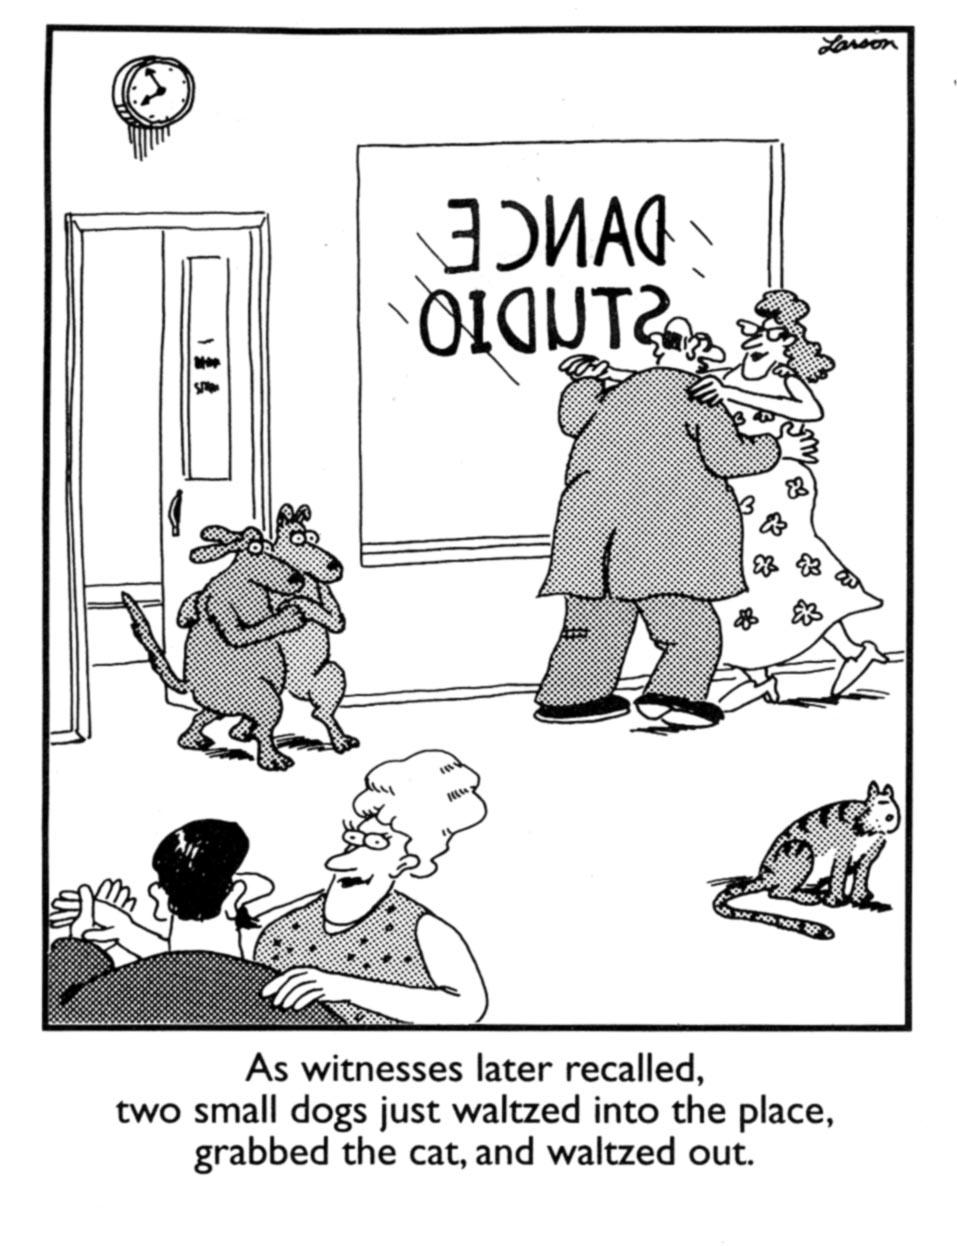
\includegraphics[width=0.5\textwidth]{graphics/example_cartoon.png}
	\caption{Cartoon by Gary Larson}
	\label{fig:fig1}
\end{figure}

The goal of this chapter is to introduce the reader into the topic of deep learning and computational humor. The motivation of this work, what the aims of this work are and as well as what methodology was applied.

\section{Motivation}

Deep learning is part of machine learning, which itself is an approach to artificial intelligence. The idea of deep learning	is to break a complex task into smaller subtasks hierarchically and let the computer learn by experience - without major human intervention. This is commonly done with neural networks which have many layers, which are commonly called deep neural networks \cite{Goodfellow-et-al-2016}.

For example: For a human to write an algorithm that reliably detects whether an image contains a dog or a cat has shown to be impossible for many years. But through convolutional neural networks this is relatively easily achievable, given there is a sufficiently large dataset of images with cats and dogs \cite{dogsvscats}. Convolutional neural networks are deep neural networks which are optimized for images \cite{cnnimg}.

Despite deep learning being a relatively new field of study there have been many advancements using this technique. In the field of self-driving cars \cite{selfdriving}, speech recognition \cite{speech}, machine translation \cite{nmt} the state-of-the-art has leaped forward to previously deemed impossible limits.

Extending this success story of deep learning into the field of computational humor is the main motivation of this work.

\section{Aim} \label{aim}
The main goal of this diploma thesis is to research whether computers are capable of understanding human humor by learning Gary Larson's cartoons (see figure \ref{fig:fig1}). This will be achieved by applying several deep learning techniques.

This work is aiming to create a dataset for computational humor. Gary Larson has created many cartoons each with an image and most with a punchline. These are annotated with a funniness rating.

The questions this work tries to answer, are the following:

\begin{itemize}
\item Which neural network architecture is best suited for predicting the funniness?
\item Does it beat simple baselines?
\item If it beats the baseline, does it really generalize the humor, or does it take cheap shortcuts?
\item Is both visual and text input the best idea for predicting the funniness? Or are they alone better?
\end{itemize}

On a higher level this thesis tries to open the field of computational humor for deep learning.

\section{Methodology}

The methodology of approaching humor using deep learning is very important and listed below.

\subsection {Literature Research}

Firstly a detailed literature research was performed. Goal was to get a grasp of the state-of-the-art of deep learning in the field of computational humor, image classification, natural language processing and human humor.


\subsection {Dataset Acquisition}
In this step the ground truth was created: A data set of Gary Larson's cartoons with funniness annotations was created. These cartoons were prepared in such a way they could be used for training the neural networks effectively. This included cropping, resizing and filtering the cartoons. Extracting the punchlines, as well as annotating the funniness.

To make this process easier an annotation tool was created. This was a web application which allowed easy preparation of cartoons.

\subsection{Development: Design, Implementation and Evaluation}

This step was iteratively done, in order to adapt to problems which occurred during implementation.

\begin{enumerate}

\item An architecture candidate was picked and designed. This was based on prior knowledge and previous literature research.
\item This architecture was implemented and trained.
\item The resulting model was evaluated. Problems were determined and possible solutions analyzed.

\end{enumerate}

At first the focus was on visual-only models. Then the focus shifted towards text-only models. Finally there were several approaches on combining both text- and visual features into a single model. Also the architectures went from simple to more complex per iteration.

The architecture candidates ranged from relatively simple convolutional neural networks to models which contain of many sub-models with an autoencoder. For more information please refer to chapter \ref{design}.

During development the trained models were applied on the validation set. The performance of the model were determined by two metrics: Accuracy and mean absolute error. 

\subsection{Final Evaluation}

Finally the most interesting models were picked and a more detailed evaluation was performed. This evaluation was done on completely new data for the model - the test set. This was done to get the true performance of the model and shows whether the model overfits. Goal of this phase was to find answers to the questions listed in section \ref{aim}.

The final conclusion was based on the findings of the final evaluation. Furthermore a  conclusion and possible future work was worked out.


\chapter{Background}

As this work combines the field of computational humor with deep learning, an understanding of both fields is required. This chapter contains the required background for this thesis.

\section{Machine Learning and Artificial Intelligence}
The field of AI tries to reproduce (human) intelligence using computers. Since it is yet impossible to develop a truly intelligent computer program, also known as strong AI. AI researchers typically pick certain subtasks of what is considered to require intelligence, also known as weak AI. For example in the beginning of AI research playing chess was considered to be a very difficult task which required intelligence. Now chess engines are able to beat every human player. The next frontier for many years was the game of Go. But eventually in 2016 AlphaGo showed that computers are able to beat the best human players in this game as well. The general assumption is that by solving each of these subtasks we get closer to strong AI, or even beyond.

\todo{Venn Diagramm das AI und ML in Relation zueinander setzt}

% https://de.wikipedia.org/wiki/K%C3%BCnstliche_Intelligenz#Starke_und_schwache_KI

Machine Learning (ML) is a field of Artificial Intelligence (AI). Given a set of training samples. In Machine Learning an ML-algorithm finds a model such that the learned model generalizes as good as possible. This model can be parametric or non-parametric. A parametric model means that the general function is fixed and can only be adjusted by adapting the parameters. For example neural networks are parametric. In contrast in a non-parametric model the function itself is constructed by the machine learning algorithm. An example for this type of model would be k-Nearest Neighbor. Since the focus of this work are neural network we will discuss parametric models in detail.

More formally, a model is a function $\boldsymbol{y}(\boldsymbol{X}, \boldsymbol{\theta})$ where $\boldsymbol{y}$ is a function, $\boldsymbol{X}$ is the training data and $\boldsymbol{\theta}$ are the parameters of the model. Through some optimization algorithm (for example gradient descent) the model is adjusted such that it generalizes ("learns") the underlying structure such that it can make predictions for previously unseen samples. Important is the distinction between model parameters ($\boldsymbol{\theta}$) and model hyperparameters. Model hyperparameters are parameters which cannot be estimated from the available data and are typically set by a human or a heuristic. In contrast, given the previously defined hyperparameters model parameters can be estimated from the data

% https://www.amazon.com/Applied-Predictive-Modeling-Max-Kuhn/dp/1461468485/ref=as_li_ss_tl?keywords=Applied+Predictive+Modeling&qid=1558557110&s=gateway&sr=8-1&linkCode=sl1&tag=inspiredalgor-20&linkId=a257735169b3234cc2247d40137cf238&language=en_US

The goal of machine learning is basically to approximate a function from data. Depending on what data is available different strategies need to be used. Typically the most convenient and preferred mode is supervised machine learning. Supervised means that not only the data $\boldsymbol{X}$ is available, but also the target values $\boldsymbol{t}$. This means that the problem can usually be relatively easily solved using an optimization algorithm (for example: gradient descent). More formally we try to find a $\boldsymbol{\theta}$ such that $\boldsymbol{y}(\boldsymbol{X}, \boldsymbol{\theta}) = \boldsymbol{t}$.

The task is called differently, depending on the possible values of $\boldsymbol{t}$. If $\boldsymbol{t}$ can take continuous values it is called a regression task. The algorithm which is used to train the model is called a regressor. If $\boldsymbol{t}$ is categorical and can only take finite values, then it is called a classification task. The algorithm which is used to train is called a classifier. An example for a regression task is stockmarket prediction, and an example for a classification task is spam detection. Important to note is, that often regression task can be modelled as classification task and vice versa. Instead of predicting the stock market directly, one can instead predict classes of <50, 51-100, 101-200, 200< and use the average value of each bucket as the predicted stockmarket. The right approach is highly task dependent.

If labels are not available then unsupervised machine learning is typically applied. For example clustering methods allow unsupervised ML. If only some labels are available semi-supervised learning may be the right mode.

The data $\boldsymbol{X}$ is a matrix where each row is a sample and each column a feature. A feature is an individual measurable property or characteristic of a phenomenon being observed \cite{bishop}. For example when trying to apply a machine learning task on an image one could use the red, green and blue channel values of each pixel as a feature. Choosing appropriate features is a difficult task and can make or break the performance of the trained model.

Important for the model $\boldsymbol{y}$ is how well it generalizes for new data. After all, getting a $\boldsymbol{y}$ which predicts the data $\boldsymbol{X}$ perfectly is trivial. If all the model does is memorizing the target labels $\boldsymbol{t}$, then the model is always right. This is called overfitting. The following method could be employed to detect overfitting:

\begin{enumerate}
\item Take the data set $\boldsymbol{X}$ and split randomly into three distinct sub sets: Training, validation and test set. The split ratio depends on the specific task.
\item Train the model on the train split.
\item Check performance of the trained model on the validation split.
\item Adjust hyper parameters such that the model generalizes better for the validation set
\item Repeat step 2, 3 and 4 until some halting criterion (for example, if the performance does not improve anymore).
\item Check final performance on the test set of the best trained model
\end{enumerate}
Note the validation/test split is only needed if there are hyperparameters which are being tweaked multiple times.
Due to the lack of standardization, sometimes the validation set is actually the test set and the test set is actually the validation set.
If this process is not adhered to it is called data leakage and it is especially dangerous if some data from the test set leaks into the training or validation set. 
This method is called the Holdout method. 

\todo{Schematische Darstellung von holdout Methode}

Another method is called Cross-validation: Here the data is randomly split into $n$ partitions. Then the $n$ models are trained for each partition, where the partition is the test set and the remaining data is used for training. If the model performs well on each partition, then it is considered that the model generalizes well.

\begin{enumerate}
\item Take the data set $\boldsymbol{X}$ and split into n partitions
\item For each partition $\boldsymbol{P}$:
\item |\quad Train the model on $\boldsymbol{X} \setminus \boldsymbol{P}$
\item |\quad Calculate performance on $\boldsymbol{P}$
\item Final performance evaluation. Commonly used is the average performance with variance.
\end{enumerate}

\todo{Schematische Darstellung von Cross validation}

Measuring the performance of a model $\boldsymbol{y}$ is an important task. Choosing the performance measure is highly task dependent. For this thesis the mean absolute error (MAE) and the accuracy were determined to be suited.

\newtheorem{mae}[DefCounter]{Definition}

\begin{mae}
$MAE = \frac{1}{n}\textstyle \sum_{i=1}^n \displaystyle\mid \hat{X}_i - X_i \mid$
\end{mae}

\newtheorem{accuracy}[DefCounter]{Definition}
\begin{accuracy}
$Accuracy = \frac{|True Positives| + |True Negatives|} {|True Positives| + |True Negatives| + |False Positives| + |False Negatives|}$
\end{accuracy}

MAE is interesting because a near miss is less penalized. For example, if a model predicts funniness of 5, while the real funniness is 6, the term $\mid 5 - 6 \mid = 1$. On the other hand if the predicted funniness were a 2, the term $\mid 2 - 6 \mid = 4$. The lower the MAE the better.

Accuracy has been chosen because it is very easy to understand and is commonly used for classification tasks. The higher the accuracy the better.



%TODO:
%optional verschiedene einfache ML Systeme erwähnen (Decision Tree, Random Forest, Naive Bayes, KNN etc.) => Wahrscheinich je nach dem wieviel Inhalt noch notwendig ist


\section{Neural Networks}

Before neural networks, there was the perceptron. It is a binary classifier and uses a linear function to perform classification. Binary means, that In its base form it can distinguish between two states. The learning process starts with a random decision boundary, which is iteratively adapted such that the number of misclassifications is minimized. Due to the linear decision boundary the perceptron is not able to learn many classes of problems. For example a simple XOR can not be learned by a basic perceptron. This motivated the use of multi layer perceptrons, since they are in theory able to approximate any function.

Historically Perceptrons are the basis for feed forward neural networks. They can be considered as multiple layers of perceptrons connected (=Multi layer perceptron). The main difference between perceptrons is that neural networks are composed of only differentiable functions, which allows for a more efficient training process.

\begin{figure}[ht]
	\centering
  	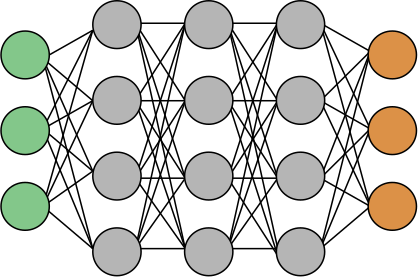
\includegraphics[width=1\textwidth]{graphics/simple_neural_network.png}
	\caption{Fully Connected Feed Forward Neural Network}
	\label{fig:feedforward}
\end{figure}

Part of the reason why neural networks are so powerful, especially deep neural networks, stems from their flexibility. They can adapt to many different domains very easily. Illustrated at Figure \ref{fig:feedforward} is a fully connected feedforward neural network with 3 hidden layers. 

A neural network generally consists of multiple neurons, layers and connections. The general inspiration for them is the human brain which also consists of similar building blocks. \\

From a different perspective, neural networks can also be seen as a series of functional transformations of some input vector into an output vector. Given the input $x_1, ..., x_D$ and $M$ connections the input layer can be described as:
\begin{equation}
a_j = \sum_{i=1}^{D} w_{ji}^{(1)}x_i + w_{j0}^{(1)}
\end{equation}

where $j = 1, ..., M$. $w_{ji}^{(n)}$ is usually referred to as weights and $w_{j0}^{(n)}$ as biases. $a_j$ is called an activation, which is then transformed using a nonlinear, differentiable activation function $h(\cdot)$:
\begin{equation}
z_j = h(a_j)
\end{equation}
Depending on the problem different activation functions are applied. Common functions are
\begin{itemize}
\item Tanh function:
\begin{equation}
h(x) = tanh(x)
\end{equation}
\item Sigmoid Function:
\begin{equation}
h(x) = \dfrac {1} {1 + e^{-x}}
\end{equation}
\item ReLU: Very often used in deep learning
\begin{equation}
h(x) = max(0, x)
\end{equation}
\item SoftMax: Does not take a single input, but multiple inputs. Can be used to transform any inputs into a probability distribution. This is commonly used for the final layer of classification tasks with multiple classes (multi class classification)
\begin{equation}
h(\boldsymbol{x}) = \dfrac{e^{x_i}}{\sum_{k=1}^{M} e^{x_k}}
\end{equation}
\item Logistic Sigmoid: Similar to SoftMax, but used for binary classification
\begin{equation}
\sigma(x) = \dfrac{1}{1 + exp(-x)}
\end{equation}
\end{itemize}


for the first hidden layer the following values are linearly combined:
\begin{equation}
a_k = \sum_{i=1}^{M} w_{kj}^{(2)}z_j + w_{k0}^{(2)}
\end{equation}

where $k = 1, ..., K$ is the total number of outputs of the first hidden layer. The same procedure is repeated for the remaining hidden layers. The final result for classification tasks is usually obtained by applying a softmax activation function of the last layer's output.

Combining these transformations together for a relatively simple two layer network results in the following equation:

\begin{equation}
y_k(\boldsymbol{x}, \boldsymbol{w}) = \sigma\left(\sum_{i=1}^{M} w_{kj}^{(2)}h\left(\sum_{i=1}^{D} w_{ji}^{(1)}x_i + w_{j0}^{(1)}\right) + w_{k0}^{(2)}\right)
\end{equation}

This term can be simplified, by assuming that the input vector $x$ has always a constant term with the value $1$. As this removes the additional addition for the bias for each layer.

\begin{equation} \label{forwardcalculation}
y_k(\boldsymbol{x}, \boldsymbol{w}) = \sigma\left(\sum_{i=1}^{M} w_{kj}^{(2)}h\left(\sum_{i=1}^{D} w_{ji}^{(1)}x_i\right)\right)
\end{equation}

Evaluating \ref{forwardcalculation} is called forward propagation.

For training a loss function $L(\boldsymbol{w})$ is defined, where $\boldsymbol{w}$ are the trained weights.

The loss can have many different forms, but in the following we will discuss primarily the cross entropy loss, since it is commonly used for classification tasks.

\begin{equation}
L(\boldsymbol{w}) = -\sum_{n=1}^N \left( t_n\,\text{ln}\, y_n + (1 - t_n)\,\text{ln}(1 - y_n)\right) \text{ where } 
y_n = y(\boldsymbol{x_n}, \boldsymbol{w})
\end{equation}

Generalized for multiclass classification with $K$ mutually exclusive one hot encoded classes:

\begin{equation}
L(\boldsymbol{w}) = -\sum_{n=1}^N \left(\,\sum_{k=1}^K \left(t_{kn}\,\text{ln}\,y_k(\boldsymbol{x_n},\boldsymbol{w})\right)\right) \text{ where } y_k(\boldsymbol{x}, \boldsymbol{w}) = \text{SoftMax}(\boldsymbol{y}(\boldsymbol{x_k}, \boldsymbol{w}))
\end{equation}

For regression tasks the L1 loss can be used:

\begin{equation}
L(\boldsymbol{w}) = \dfrac{1}{N} \sum_{n=1}^N |x_n - y_n| \text{ where } 
y_n = y(\boldsymbol{x_n}, \boldsymbol{w})
\end{equation}

The goal of training neural network is to minimize the loss of the model:

\begin{equation}
\text{arg min}\quad L(\boldsymbol{w})
\end{equation}

Training takes advantage of the fact that it is a function composition of differentiable functions. This allows the use of a technique called gradient descent. The idea is intuitive: Walk along the path with the steepest descent until some halting criterion is met. Because the neural network is differentiable the steepest descent is relatively easily obtained, by taking the negative of the first derivative of the loss function. A halting criterion could be number of iterations, diminishing or no improvements over time or reaching some predefined threshold.

A pseudo code for gradient descent:

\begin{enumerate}
\item Compute gradient: $\boldsymbol{w}' = \bigtriangledown	L(\boldsymbol{w})$
\item Update weights: $\boldsymbol{w} := \boldsymbol{w} - \alpha \boldsymbol{w}'$
\item Repeat steps 1 and 2 until halting criterion is met

\end{enumerate}

$\alpha > 0$ is a hyperparameter and called the learning rate. $\alpha$ is usually set empirically and usually $0.000001 \leq \alpha < 1.0$. A too high learning rate (for example $\alpha = 1$) means that the loss of the neural network could increase instead of decrease, since it might skip important extremes. In general, the higher $\alpha$, the faster the gradient descent converges. Reversely the lower $\alpha$ the more local optimas are considered. Usually in the beginning of training the learning rate should be higher and at the end the learning rate should be lower. This is the reason why it is common to make the learning rate decay during training.


\subsubsection{Applying neural networks}
The naive implementation of gradient descent has problems, which can be mitigated by different measures:

Usually a technique called momentum is applied. A real world analogy would be a ball rolling down a hill: Over time it builds up velocity and slows down when the hill gets more shallow. This makes the gradient descent algorithm to be less prone for local minima and usually makes it converging faster to the desired optimum.

Another technique is called minibatching: Here instead of taking the gradient of the entire data set $\boldsymbol{X}$, a small subset of $\boldsymbol{X}$ is taken. This not only reduces the amount of computation needed, but also makes it such that local minima are less of a problem.

Obtaining the gradient is also a computationally complicated step. The usual forward derivation method commonly learned in school does not scale well for many parameters. Therefore a technique called backpropagation is commonly used. [TODO]

One problem of every machine learning algorithm, and especially for neural networks is the problem of overfitting. There are different measures available to counteract overfitting.

The main three approaches we will discuss here are: Regularization, Data augmentation, early stopping and Dropout layers. 

The idea of data augmentation is to synthetically increase the size of the dataset by applying several transformations on the original data. All transformations must not alter the original label of the sample. For examples, image data usually allows many different kind of filters and transformations to be applied. Common operations are random crop, random rotation and add synthetic noise.

Regularization tries to avoid overfitting by penalizing	high weights of neurons. This avoid certain inputs from dominating outputs and nudges the network to make use of all inputs. This can easily be achieved by adapting the loss function slightly:

\begin{equation}
L_{reg}(\boldsymbol{w}) = \dfrac{\delta}{2}\norm{\boldsymbol{w}}^2 + L(\boldsymbol{w})
\end{equation}

where $\delta$ is called weight decay and usually $0.000001 \leq \delta \leq 0.0001$.

Another simple technique is early stopping. The idea is simple: Remember the best performing model $y_{val}$ on the validation set, instead of the final model $y$ after gradient descent terminated. After training has finished return $y_{val}$ instead of $y$.

Finally a dropout layers can be used. The idea is similar to regularization: The network should not overly rely on certain inputs. A dropout layer turns off neurons with a certain probability. This forces the network to generalize better. Usually in CNNs dropout layers are placed at the end of the network before the last fully connected layer.

\todo{Schematische Darstellungg von Dropout}

Due to the sheer amount of hyperparameter and possible approaches, successfully designing and training a neural network can be a challenging task. There are many rules of thumbs for many hyperparameters and class of problems but in the end it is in the end of the developer to use a good mixture of clever tricks, as well as trial and error.

The design of the neural network also influences how much it tends to overfit. As a rule of thumb, the more neurons a neural network has, the bigger the learning capacity of the neural network and the more easy it overfits if the dataset is not sufficiently large. Empirically deep networks (many layers) have shown to generalize better compared to less deep networks but with similar number of neurons.

\subsubsection{Deep Learning}

If a neural network is used with multiple layers, where each layer applies some form of higher level feature extraction compared to the earlier layers it is called deep learning. Such neural network is also called a deep neural network.

An advantage of deep neural network is that they scale very well with the size of the dataset and with the amount of computation available. As the computational power increases and the size of the datasets as well, the performance of models deep learning may enable also increases.

Multiple layers in neural networks have been existing for many years, but just in relative short time this field gained a lot of traction. There are two main reasons for this: General purpose programming of graphics cards and clever neural network architectures.

One big problem of training deep neural networks is, that it is very computationally expensive. Backpropagation reduces the required power significantly, but for models with many million parameters it is still infeasible to train them on weak hardware. An advantage of training neural networks is that it can be highly parallelized. This in combination with the fact that graphics cards started to be programmable caused a significant leap in feasible neural network architectures.

Another innovation necessary for the breakthrough of deep neural networks was the introduction of clever architectures. Through convolutional layers the number of parameters trained decreases significantly, compared to a multi layer perceptron with the same number of layers.

\subsubsection{Convolutional Neural Networks} \label{mlcnn}

Based on feedforward neural networks convolutional neural networks emerged. A convolutional neural network (CNN) is a deep neural network, since it consists of multiple hidden layers, where additionally to fully connected hidden layers there are usually several pooling and convolutional layers.

Convolutional layers apply a convolution on each pixel. A convolution is a weighted sum between two functions. The first function is the input signal and the second function a filter kernel. Instead of each neuron being connected to all other neurons, they are connected to a relatively small local subset of the neurons in the previous layer, which allows them to recognize certain local patterns (for example edges). This pattern is called a kernel. The kernel is shared among the input neurons (Parameter Sharing). This introduces translation invariance, which means that it matters less if a feature occurs at the center or on the edges of an images. Additionally to increase the capacity, usually multiple convolutions with learned kernels are applied per layer. This is called the depth of a layer.

Pooling layers are applied after convolutional layers. Their goal is to reduce the dimensionality of the data. Local pooling layers are connected to a local subset of the neurons in the previous layer, but without weights, biases or a kernel. The input is transformed by a function. A typical pooling layer is max pooling, where the result is the maximum value of all incoming connections of the current local subset (for example 2x2). Another form of pooling is global pooling, where the entire data is pooled at once, this is usually employed at the end of the convolutional part of a CNN.

Fully connected layers are usually the last layers of a CNN, their task is to perform classification based on the extracted features of the previous layers. Interestingly the convolutional part of a CNN can be used for another tasks with good performance, more about this at section \ref{transferlearning}.

\begin{figure}[ht]
	\centering
  	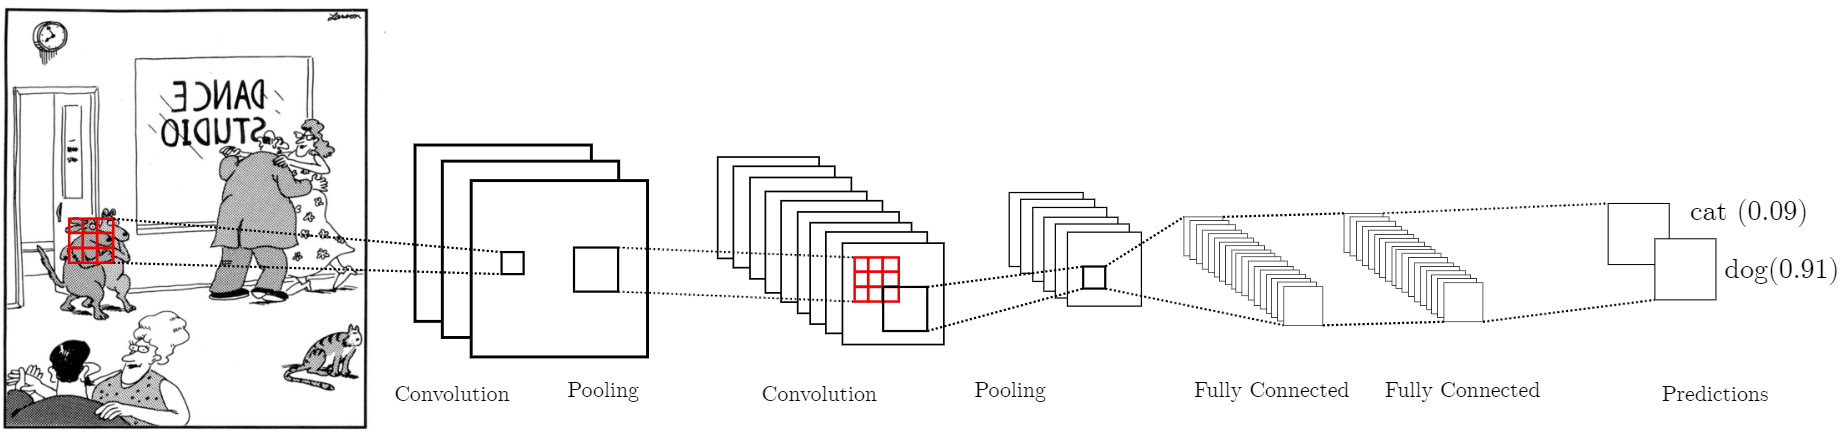
\includegraphics[width=1.0\textwidth]{graphics/cnn.png}
	\caption{Visual representation of a convolutional neural network}
	\label{fig:feedforward}
\end{figure}
\pagebreak

\todo {Graphische Darstellung eines Convolution Layers}
\todo {Graphische Darstellung eines Max Pooling Layers}

\subsubsection{Recurrent Neural Networks}
Recurrent Neural Networks allow neural networks to be applied on sequences, by allowing cycles in the topology of the network. Usually a recurrent neural network (RNN) consists of multiple units, such as Long Short-Term Memory (LSTM) units or gated recurrent units (GRU) \cite{gru}.

Each architecture has different benefits and applicable domains. Even among LSTM networks there are many variations. One of the reasons why LSTMs are so powerful compared to other architectures is due to their design, as it avoids the vanishing/exploding gradient problem of regular RNNs \cite {vanishinggradient}.

The simplest LSTM unit consists of a memory cell with input and output gates. Inside the LSTM a self-recurrent connection is placed and the vanishing gradients are kept inside by the gates. For a more detailed architecture overview Long Short-Term Memory by Hochreiter Schmidhuber is recommended \cite{hochreiter}.

\todo {Schematische Darstellung eines simplen RNNs}
\todo {Schematische Darstellung einer LSTM Zelle}

\subsubsection{Autoencoder}

An autoencoder is a deep neural network which learns a compact representation of data similar to principal component analysis in an unsupervised way. An autoencoder consists of two parts: The encoder and decoder. The encoder performs a dimensionality reduction from a high dimensional data to a low dimensional representation. The decoder on the other hand tries to reconstruct the original data from the low dimensional representation.

\todo {Schematische Darstellung eines Autoencoders}


%TODO:

%Grundlagen von NN Design. => Welche Hyperparameter muss man tunen und was sind sinnvolle Werte (Learning Rate, Layer, anzahl Neuronen, Weight Decay, etc.) 

%Wenn noch Platz: Backpropagation erklären

\section{Natural Language Processing}
Natural Language Processing (NLP) is a subfield of artificial intelligence and linguistics where the goal is to build computer programs which are able to understand human language. Common tasks of NLP include part-of-speech tagging, paraphrase identification, machine translation and speech recognition.

Early NLP tried to achieve its goal by building traditional parsers, similar to what compilers to for programming languages. The problem was that these techniques are inadequate for human languages, due to their ambiguity.

Another common approach has been to apply traditional machine learning for NLP. The idea here is to extract certain features of a dataset of text and using these features train a classical machine learning model using, for example, a support vector machine.

The current state-of-the-art results in NLP are achieved by applying deep learning to this field. An advantage of many text domains, is that there is lots of data available. This is a big advantage especially for unsupervised methods, as no difficult labelling must be performed.

For both traditional machine learning and deep learning based natural language processing it is important to extract the right features from text. A trivial approach would be giving each word a unique identification number. The problem with this approach is that one loses the entire semantic information about the words. The words king and queen are more similar than king and house. Keeping this information is crucial for successful natural language processing.

This is where vector space models are often applied. The idea is to represent each word in a high dimensional vector space, where a certain similarity measure holds.

There is the concept of positive similarity, denoted using the $\otimes$ operator. And there is the concept of negative similarity, denoted using the $\overline{\otimes}$ \cite{TUW-233295}. Similarities based on the dot product are positive similarity measures. Commonly used is the cosine similarity. While similarities based on distance are negative similarity measures, for example the euclidean distance. CNNs and other neural network architectures are based on positive similarity, as they perform a convolution which applies the dot product across the data.

These vector representations are also called word embeddings. There are many different techniques to obtain such embeddings. A very simple, but successful technique is called TFIDF, another common approaches are Word2Vec and GloVe embeddings. One problems of these embeddings are, that they mostly ignore the context of the word. The word bank has different meanings, depending on if the current topic is about rivers or about money. This problem is what the most successful embeddings to date tackle: They consider the context of the word (sentence) to obtain a better vector representation.

In the following sections the embeddings which were used during in this thesis are discussed.

\subsubsection{TFIDF}
TFIDF stands for term frequency inverse document frequency and is a simple, but powerful vector space model. The idea originated in information retrieval where  TODO

\subsubsection{GloVe}
TODO

\subsubsection{ELMo}
TODO


% TODO
%Verschiedene gängige Aufgaben aus NLP erklären (Sentiment Analysis, POS Tagging, machine translation, Paraphrase Identification etc.)


\section{Transfer Learning} \label{transferlearning}

Usually, the more complex a given task is, the more labelled data deep learning needs to achieve good results. This is not only expensive, but sometimes not possible. For example, Gary Larson has only drawn so many cartoons in his lifetime. Labelling a big data set is also a big challenge and not always feasible.

This is why transfer learning is applied: Instead of training a completely new model for each problem task, the idea is to reuse models and only slightly adapt them for new tasks. The original model can be trained on an already existing big dataset and the fine tuning does not need as big of a dataset. The finetuning in the context of deep neural networks is often done by fixating the weights of neurons in certain layers during training. Usually these layers perform more general feature extraction, which is better applicable to other domains.

For example there are already very big datasets for image classification tasks. Training a good performing classifier on these datasets has already been done numerous times. Especially CNNs have an architecture very suited for transfer learning: As mentioned in [\ref{mlcnn}], there is the convolutional part and the fully connected part. Usually the convolutional part is acting as a feature extractor and the fully connected part makes the final prediction. Empirically it has been shown that the feature extractor generalizes often very well to new domains. Depending on how similar the domain is less training is needed for the new domain. This paper used a pretrained ResNet8 model which has very good performance for traditional image classification tasks and applied it on Gary Larson's cartoons.

For natural language processing a similar breakthrough compared to the CNN architectures probably happened just recently with new word embedding techniques, such as ELMo and BERT. What true potential these techniques have has yet to be shown. Importantly these word embeddings transfer well for a broad range of tasks [TODO] while reaching state-of-the-art performance. 

% TODO:
%Herausforderungen von Transfer Learning

\section{AutoML}
Definition

Wozu?

Methoden zu AutoML

\section{Computational Humor}
definition of computational humor

Problematik von Humor für Computer erklären

language understanding

traditional approaches of computational humor

WordNet 

Stichprobenartig Papers wiedergeben, zB: 

https://ieeexplore.ieee.org/stamp/stamp.jsp?tp=\&arnumber=1613822

https://www.ijcai.org/Proceedings/03/Papers/009.pdf

\section{Related work}

Den Text aus dem Proposal übernehmen und die einzelnen Paper noch genauer beschreiben:

Previous approaches of computational humor mainly focused on written text \cite{Yang2015HumorRA}\cite{Bamman2015ContextualizedSD}\cite{HumoristBot}. Research of humor using deep learning is still in its infancy. With the advent of deep learning and convolutional neural networks (=CNN) in recent years \cite{Druzhkov2016}, images may now be taken into consideration as well. Similarly deep learning enabled modern language embeddings such as ELMo \cite{elmo} and BERT \cite{bert} to achieve state-of-the-art results on various natural language processing tasks. Given these advances there is a possibility that humor may be more tractable using deep learning compared to other methods.
\todo{Ihr Text hier.}


\chapter{Design} \label{design}

In this chapter the design process of tackling of understanding Gary Larson's cartoons using deep learning is outlined.


\section{Dataset Acquisition}
The dataset consists of 2487 cartoons. Each sample consists of a cartoon image, punchline text and a funniness scale from 1 to 7. The funniness scale is ordinal, where 1 means not funny at all and 7 is very hilarious.

Annotation was performed by one of the authors (Robert Fischer) over the course of half a year. The annotation was split in two steps. The first step was preparing the cartoons. In this step the cartoons where cropped and rotated accordingly. The punchline was transcribed from the image into text format, using an OCR, but many manual adjustments had to be applied as well. Additionally cartoons with bad quality, as well as duplicates were also removed.

The second step was to annotate the funniness of the cartoons. There was the problem of humor fatigue: After annotating cartoons for too long, the annotations would get unreliable and could possibly be wrongly classified. This was mitigated by limiting the duration of the annotation sessions. Each annotation session lasted 30 minutes at maximum, but shorter sessions were preferred. 

\section{Dataset Analysis}

The dataset analysis revealed several interesting facts about the dataset. Figure [\ref{fig:labeldistr}] shows a bar plot of the label distribution. Unexpectedly the funniness is not uniformly distributed. Over 14\% of the cartoons were deemed to be not funny at all, while only 2\% of cartoons were deemed to be very hilarious.

To verify that the distribution of the annotations has not changed over the course of annotation refer to figure [\ref{fig:boxplottime}]. Each cartoon has an ascending identification number. Cartoons were  combined into buckets by this number. Finally for each of this bucket a box plot is plotted. This shows no significant change of label distribution over the course of annotation.

\begin{figure}
	\centering
  	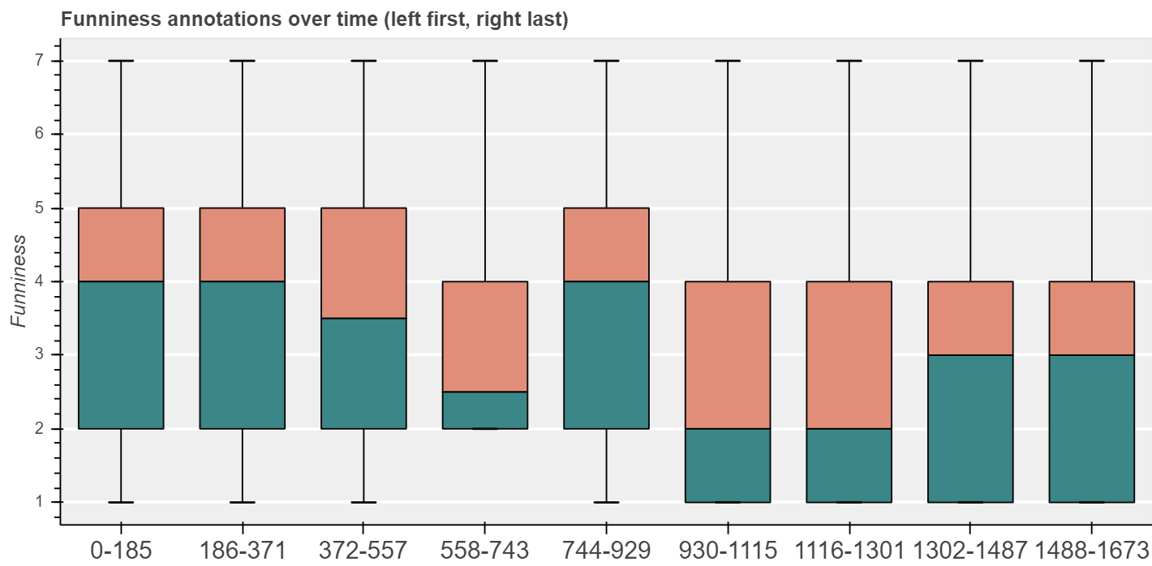
\includegraphics[width=1.0\textwidth]{graphics/average_funniness_over_time}
	\caption{Box plots of the average funniness over time in the training split.}
	\label{fig:boxplottime}
\end{figure}

A word count analysis showed that there are significant difference in the frequency of certain words. These words seem to contain certain connections to a cartoon theme. For example one of the most frequent words for funniness class 7 is "Thag" which is a common name for cartoons set in the stone age. A similar phenomena could also be observed for word phrases. For example the phrase "thousand more year" is also primarily associated with cartoons set in the stone age. A model could learn this preferences and use it to predict the funniness of a cartoon. For detailed plots please refer to figure [\ref{fig:wordocc1}], [\ref{fig:wordocc2}], [\ref{fig:phraseocc1}] and [\ref{fig:phraseocc2}].

\begin{figure}
\centering

\begin{subfigure}[b]{0.45\textwidth}
\centering
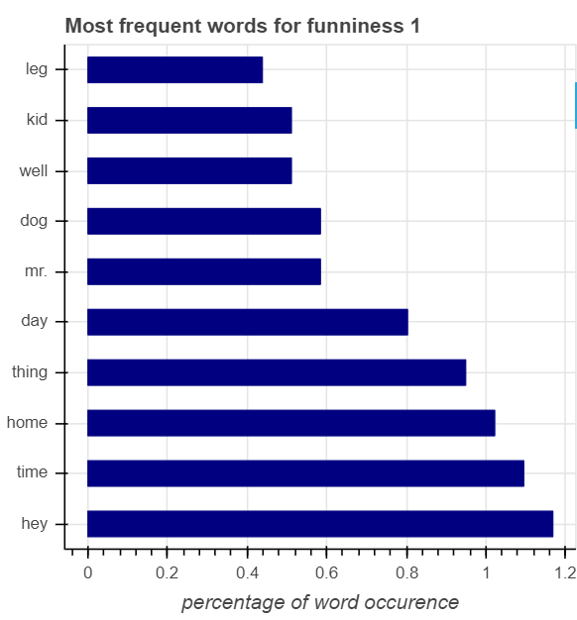
\includegraphics[width=1.0\textwidth]{graphics/word_occurence/funniness_1}
\end{subfigure}\quad
\begin{subfigure}[b]{0.45\textwidth}
\centering
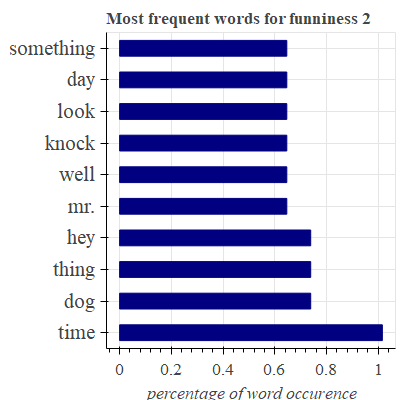
\includegraphics[width=1.0\textwidth]{graphics/word_occurence/funniness_2}
\end{subfigure}

\begin{subfigure}[b]{0.45\textwidth}
\centering
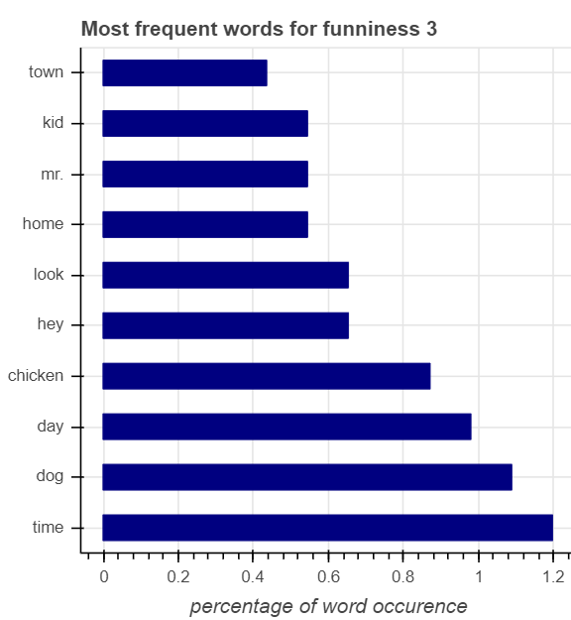
\includegraphics[width=1.0\textwidth]{graphics/word_occurence/funniness_3}
\end{subfigure}\quad
\begin{subfigure}[b]{0.45\textwidth}
\centering
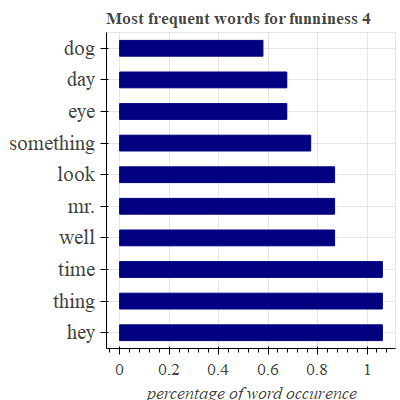
\includegraphics[width=1.0\textwidth]{graphics/word_occurence/funniness_4}
\end{subfigure}


\caption{Most frequent nouns per class 1, 2, 3 and 4.}
\label{fig:wordocc1}

\end{figure}

\begin{figure}
\centering

\begin{subfigure}[b]{0.45\textwidth}
\centering
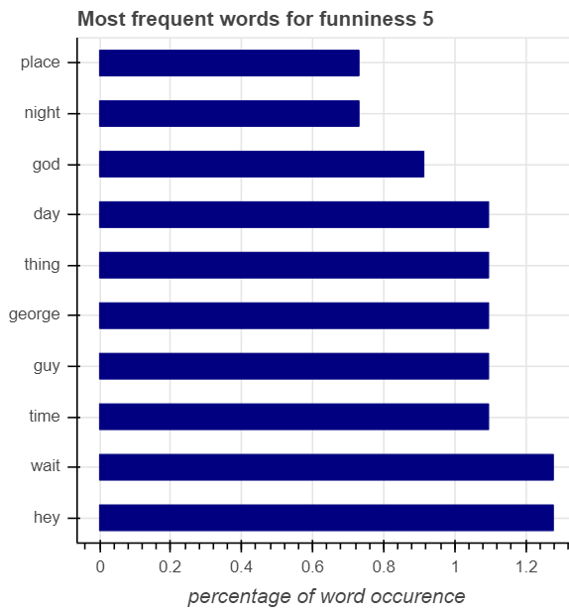
\includegraphics[width=1.0\textwidth]{graphics/word_occurence/funniness_5}
\end{subfigure}\quad
\begin{subfigure}[b]{0.45\textwidth}
\centering
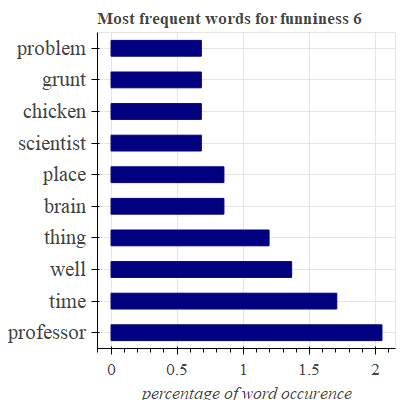
\includegraphics[width=1.0\textwidth]{graphics/word_occurence/funniness_6}
\end{subfigure}


\begin{subfigure}[b]{0.45\textwidth}
\centering
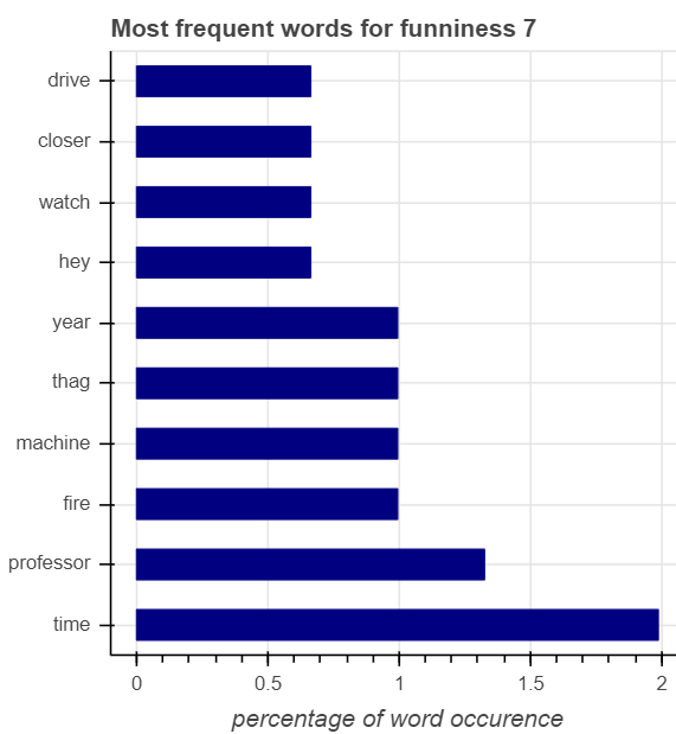
\includegraphics[width=1.0\textwidth]{graphics/word_occurence/funniness_7}
\end{subfigure}

\caption{Most frequent nouns per class 5, 6 and 7.}
\label{fig:wordocc2}

\end{figure}

\begin{figure}
\centering

\begin{subfigure}[b]{0.45\textwidth}
\centering
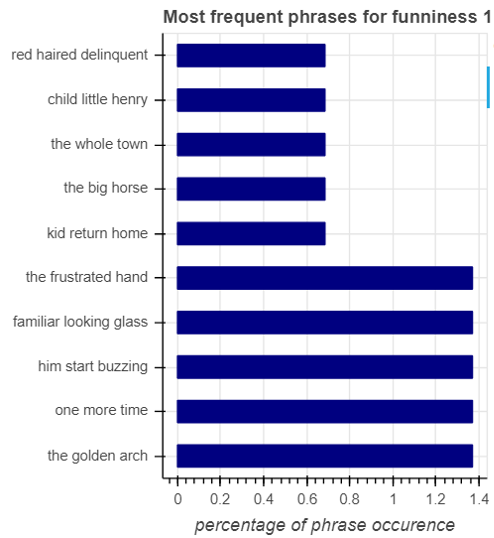
\includegraphics[width=1.0\textwidth]{graphics/phrases/funniness_1}
\end{subfigure}\quad
\begin{subfigure}[b]{0.45\textwidth}
\centering
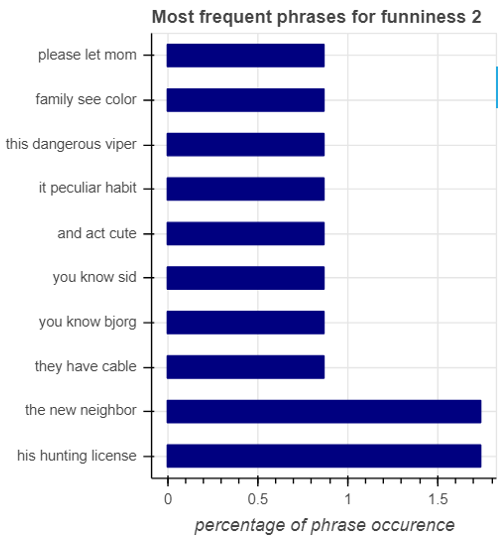
\includegraphics[width=1.0\textwidth]{graphics/phrases/funniness_2}
\end{subfigure}

\begin{subfigure}[b]{0.45\textwidth}
\centering
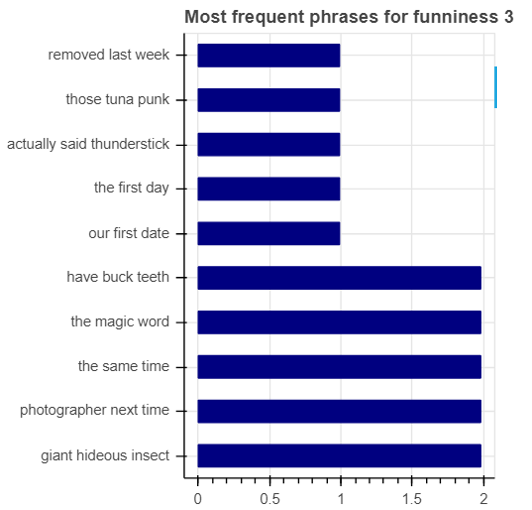
\includegraphics[width=1.0\textwidth]{graphics/phrases/funniness_3}
\end{subfigure}\quad
\begin{subfigure}[b]{0.45\textwidth}
\centering
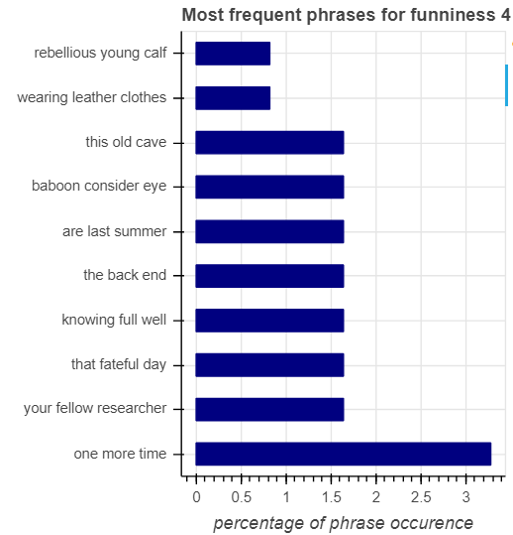
\includegraphics[width=1.0\textwidth]{graphics/phrases/funniness_4}
\end{subfigure}


\caption{Most frequent phrases per class 1, 2, 3 and 4.}
\label{fig:phraseocc1}

\end{figure}

\begin{figure}
\centering

\begin{subfigure}[b]{0.45\textwidth}
\centering
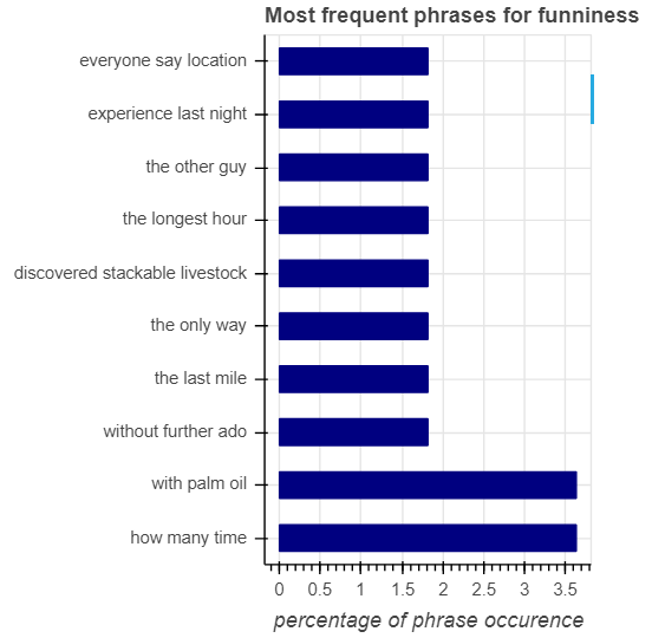
\includegraphics[width=1.0\textwidth]{graphics/phrases/funniness_5}
\end{subfigure}\quad
\begin{subfigure}[b]{0.45\textwidth}
\centering
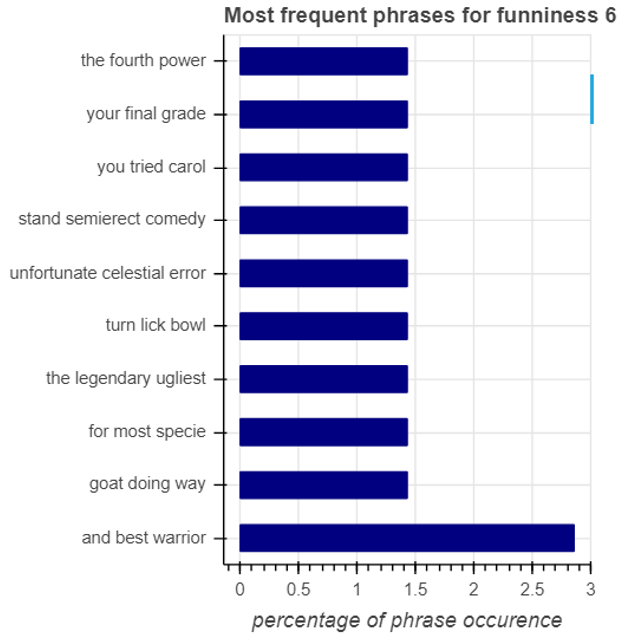
\includegraphics[width=1.0\textwidth]{graphics/phrases/funniness_6}
\end{subfigure}


\begin{subfigure}[b]{0.45\textwidth}
\centering
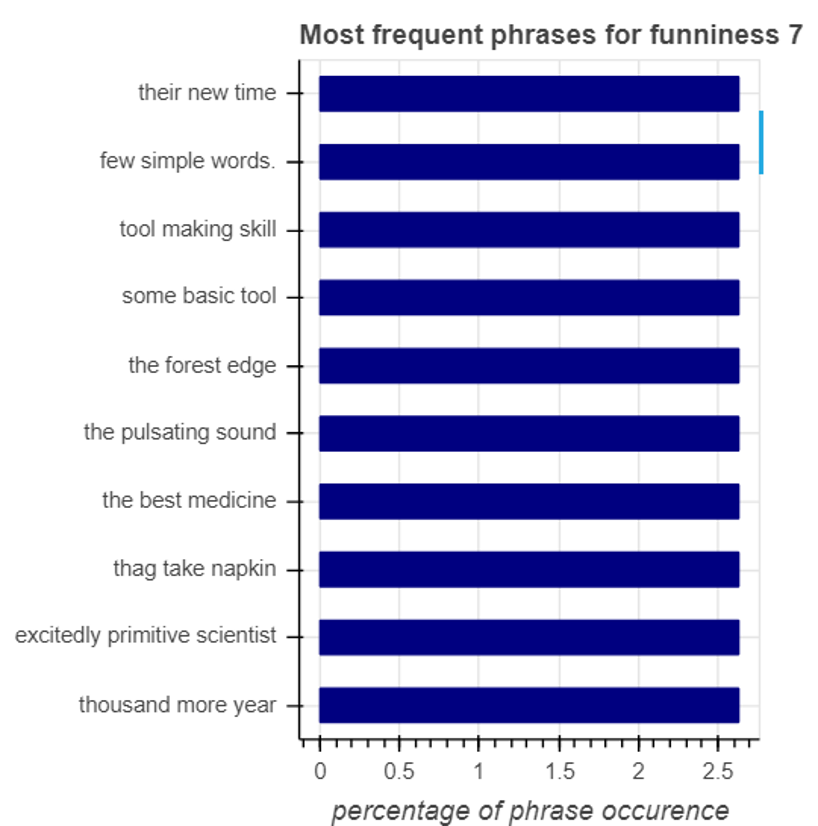
\includegraphics[width=1.0\textwidth]{graphics/phrases/funniness_7}
\end{subfigure}

\caption{Most frequent phrases per class 5, 6 and 7.}
\label{fig:phraseocc2}

\end{figure}

\section{Task modelling}

The task at hand (predicting the funniness of a cartoon) can be modelled in two ways: 
\begin{itemize}
\item Classification: Each cartoon funniness belongs to a distinct class
\item Regression: Each cartoon funniness is a sample of a continuous space
\end{itemize}

The main difference when modelling a task as a regression task versus a classification task is the final output layer and the loss used. When modelling a task as a classification problem the final layer is generally one-hot-encoded. In contrast for a regression problem the final layer is a single value. \\

Another important decision to be made is which loss function to be used. For this problem mainly cross entropy loss for classification and L1 loss for regression has been used \cite{crossentropyloss} \cite{lossfunctions}.

\section{Simple CNN}

The initial approach was to use an off-the-shelf Convolutional Neural Network (CNN) design. This neural network architecture has proven to be very effective for various image classification tasks \cite{dogsvscats}.

Wie wurde die größe des Input Layers definiert

Visuelle Illustration des finalen Netzwerks

\section{Transfer Learning CNN}

Welche Architektur wurde verwendet (ResNet18). Wieso? => Weil bereits erfolgreich für andere Tasks und bereits bei PyTorch dabei

Was wurde transferiert? Freezing von Parametern?

Visuelle Illustration des finalen Netzwerks

\subsection{Transfer Learned Object Detection}

Idee (Object Detection Model an stark transformiertem Datenset trainieren und hoffen dass es auf Gary Larson transferierbar ist => Dadurch Featurevektor von Cartoon erhalten)

Evtl. Beispiel zeigen wie so ein Featurevektor eines Cartoons aussehen könnte

Graphische Darstellung

Annotieren eines Validationdatensets um performance zu überprüfen

\section{ELMo}

\if false
The punchline of a cartoon will be converted into text strings. Humans are able to understand this representation of text quite well, but only after spending many years of learning to read. The neural network itself does not understand the semantic meaning, the encoding is arbitrary. The string "animal" has as much semantic meaning as the string "foobar". Hence training on this encoding is not expected to have good results. \\

To solve this problem Word Embeddings can be computed. These place words into a feature space where similar words are near to each other, while dissimilar words are far from each other. Such an embedding can be calculated using a Skip-Gram model \cite{wordembedding} or pretrained models are available \cite{pennington2014glove}.
\fi

Zuerst LSTM/GRU und dann sentence embedding probiert.

ELMo vs BERT? Wieso ELMo

Visuelle Illustration des finalen Netzwerks

\section{AutoML}
Wieso AutoML

Verschiedene Features (TFIDF, Glove, ELMo, TFIDF + Glove, TFIDF + ELMo)

\section{Two Stage Model}

1. Stage: 1 vs rest classifier erklären

2. Stage: Finale Regression erklären

Kombinieren von visual + text erklären

Klassen Imbalance durch 

Autoencoder Ansatz

Visuelle Illustration des finalen Netzwerks

\section{Additional Experiments}
A list of experiments performed but did not make the cut for a more detailed analysis:

\begin{itemize}
\item \textbf{LSTM / GRU}: Overfitting was a big problem early on
\item \textbf{Wasserstein Loss instead of Cross Entropy Loss}: Idea was to penalize near misses less.
\item \textbf{L1 Loss}: Model as a regression task. Model was not even able to approximate the Average Baseline using this approach
\item \textbf{Applying a discrete cosine transformation (DCT)}: Since convolutions are not well suited for line drawings the idea was to apply a DCT beforehand. 
\item \textbf{Advanced Two Stage Model}: Add different binary classifiers in the first stage.
\item \textbf{Loss Weighting of Two Stage Model}: Try different penalties for different kind of errors in the first stage. For example add more penalty for true positives compared to false negatives.
\item \textbf{Preprocessing of cartoons}: Apply different filters on cartoons. For example: Canny edge detection.
\item \textbf{Word vector combinations}: Many different word vector combinations of TFIDF, GloVe and ELMo. 
\end{itemize}

Hier muessen eventuell Sachen rausgenommen werden die doch erwaehnt wurden bzw. worden sind.

\chapter{Implementation}

Wahl der Libraries: PyTorch, pandas, sklearn, Python, etc.

Annotierungsapplikation erklären. Hat es sich gelohnt?

Architektur (Command Line via parameter steuerbar)

Wie wurden die neuronalen netzwerke gedebuggt bei Fehlern: Am meisten hilffreich war als ich die bilder durch ziffern ersetzt habe die die das label enthielten.

Welche Probleme sind aufgetreten: Fehlerhafter Split zwischen Training/Test/Validation

für visuellen teil:

Datenmanagement: Klassendiagram und erklärung

Evaluationsystem: Klassendiagramm und erklärung

Reproduzierbarkeit?

Für textteil: AllenNLP verwendet. Erklärung des Frameworks 

Conclusio der Implementierung: Kein Overengineering. Effektives Code wieder verwenden schwer mit Machine Learning

\chapter{Evaluation}

This chapter aims to evaluate the performance of the implemented architectures. In
general the results show that this problem is very hard. Despite the progress in the field of Deep Learning it was not possible to beat the baseline. \\

The cartoon data set is split into three sub sets:

\begin{itemize}
\item Training Set: 1492 samples (70\%)
\item Validation Data: 746 samples (20\%)
\item Test Data: 249 samples (10\%)
\end{itemize}

The experiments were run on a PC running Ubuntu 18.04 LTS using PyTorch 1.0 and
Python 3.6. The hardware is a GTX 1070 Max-Q with an Intel Core i7-8750H. For more
information regarding the build set up and necessary environment please refer to the GitHub Repository \cite{deephumorrepo}.

The hyperparameters were chosen based on best practice and previous
experience by the author with deep neural network training. Because there are many hyperparameters an automated search of the hyperparameter space is infeasible with the hardware available to the author.

\section{Architectures}
Several architectures have been implemented and are evaluated in the following sections.


\subsection{Baseline}

Four baseline strategies have been selected: 

\begin{itemize}

\item Most Frequent Baseline: Picks the most frequent label in the dataset.
\item Average Baseline: Returns the average funniness of the dataset. For the accuracy metric the average is rounded using round to nearest integer.
\item Random Baseline: Returns a random funniness picked uniformly from one to seven.
\item Stratified Baseline: Returns a funniness sampled from the distribution of the
training set.

\end{itemize}

For the mean absolute error metric the average performed best, while for the accuracy score the most frequent class has the best score.

\subsection{Simple CNN}
The simple CNN architecture overfits very quickly. The accuracy and MAE scores are very similar to the most frequent baseline, which indicates that the model most likely learns to return the most frequent class.

\subsection{Transfer Learning of Pretrained ResNet18}
Noteworthy about this approach is that also enabling the data augmentation in the testing/validation phase makes this approach better than the baseline. The exact reason is not obvious, but indicates that the model expects the cartoons to be augmented.

The data augmented version of this experiment unexpectedly achieved the best results during testing phase.

Sampling for each class a cartoon and examining the output layer of the trained neural network reveals some interesting insight about how the model works. In general the results show, that the classifier never assigns high confidence into the predictions. No classification assigns a probability higher than 40\%.

When examining the distribution across the different predictions over the different samples it seems that the general distribution does not change significantly. Some deviations are present, for example when comparing the probabilities for funniness 2.

In general it seems that the model often ignores the input data and instead learns the label distribution. The similarities between the predictions and the histogram of funniness occurrences are very high. Compare figure [\ref{fig:figdistr1}] and figure [\ref{fig:figdistr2}] with figure [\ref{fig:labeldistr}].

\begin{figure}
\centering

\begin{subfigure}[b]{0.45\textwidth}
\centering
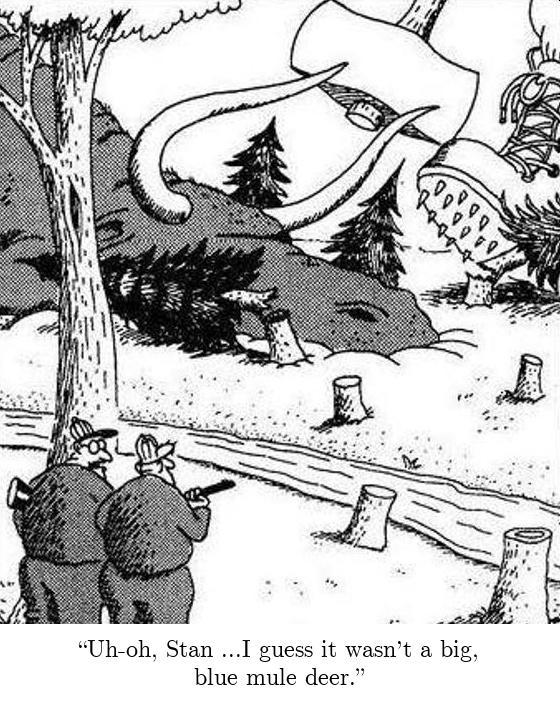
\includegraphics[width=0.9\textwidth,height=0.3\textheight,keepaspectratio]{graphics/detail/Test_for_Image_1_cartoon} \\
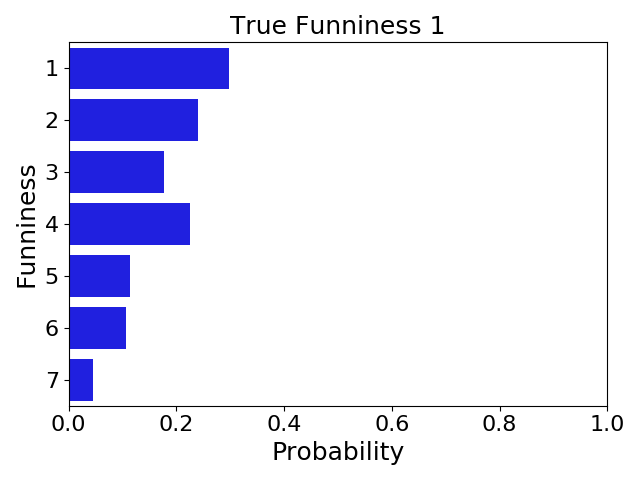
\includegraphics[width=1.0\textwidth]{graphics/detail/Test_for_Image_1}
\end{subfigure}\quad
\begin{subfigure}[b]{0.45\textwidth}
\centering
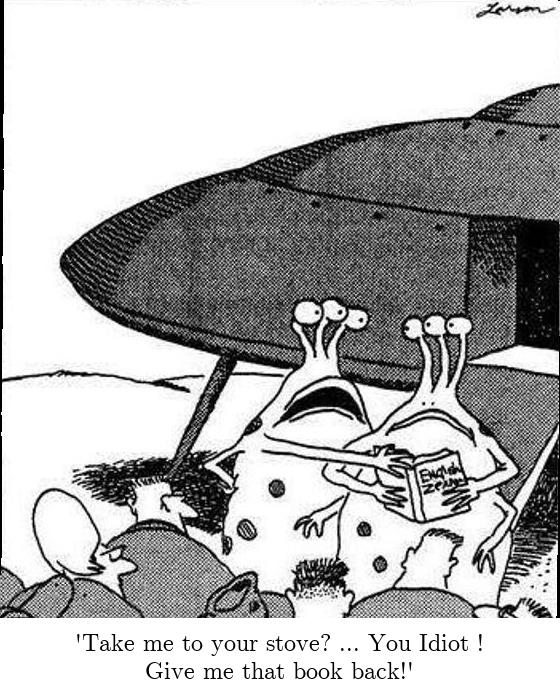
\includegraphics[width=0.9\textwidth,height=0.3\textheight,keepaspectratio]{graphics/detail/Test_for_Image_2_cartoon} \\
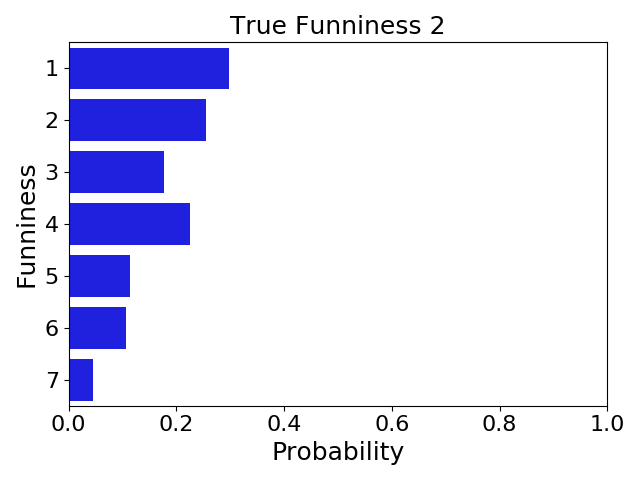
\includegraphics[width=1.0\textwidth]{graphics/detail/Test_for_Image_2}
\end{subfigure}

\begin{subfigure}[b]{0.45\textwidth}
\centering
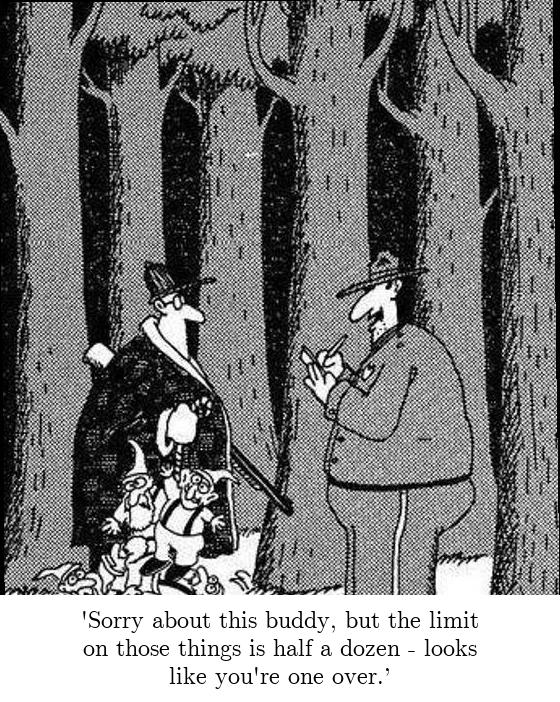
\includegraphics[width=0.9\textwidth,height=0.3\textheight,keepaspectratio]{graphics/detail/Test_for_Image_3_cartoon} \\
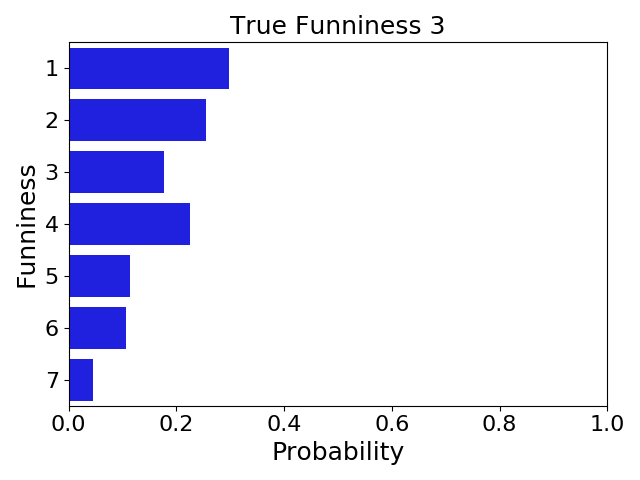
\includegraphics[width=1.0\textwidth]{graphics/detail/Test_for_Image_3}
\end{subfigure}\quad
\begin{subfigure}[b]{0.45\textwidth}
\centering
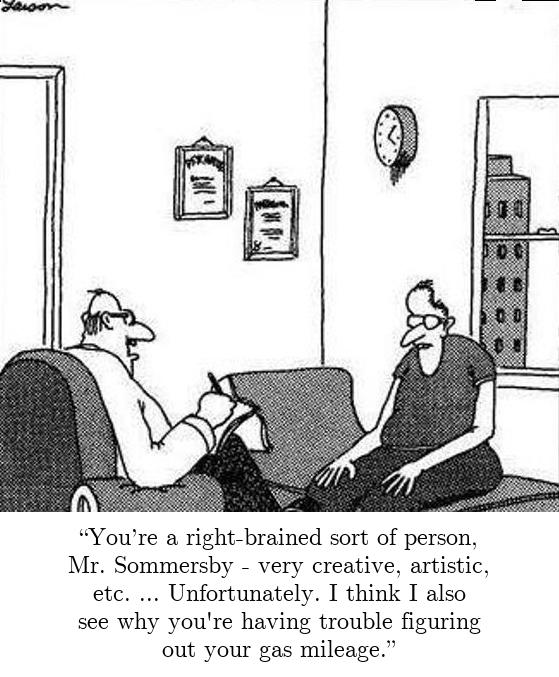
\includegraphics[width=0.9\textwidth,height=0.3\textheight,keepaspectratio]{graphics/detail/Test_for_Image_4_cartoon} \\
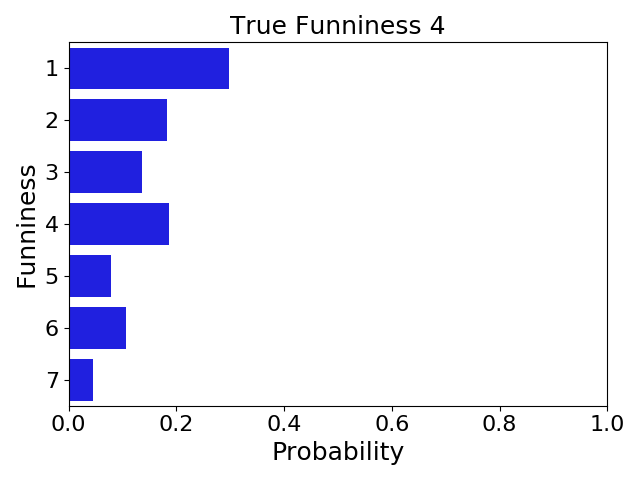
\includegraphics[width=1.0\textwidth]{graphics/detail/Test_for_Image_4}
\end{subfigure}

\caption{For the classes 1, 2, 3 and 4: The bar plots represent the probability the classifier assigned each category for the cartoon above.}

\label{fig:figdistr1}

\end{figure}


\begin{figure}
\centering

\begin{subfigure}[b]{0.45\textwidth}
\centering
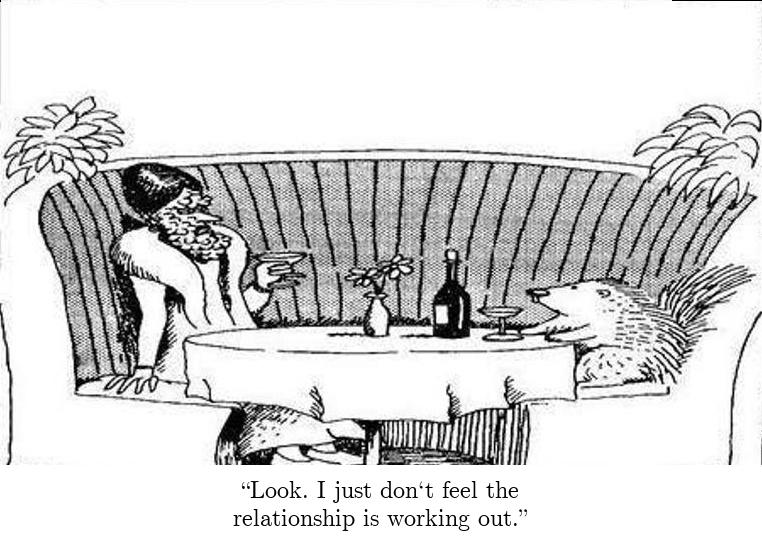
\includegraphics[width=0.9\textwidth,height=0.3\textheight,keepaspectratio]{graphics/detail/Test_for_Image_5_cartoon} \\
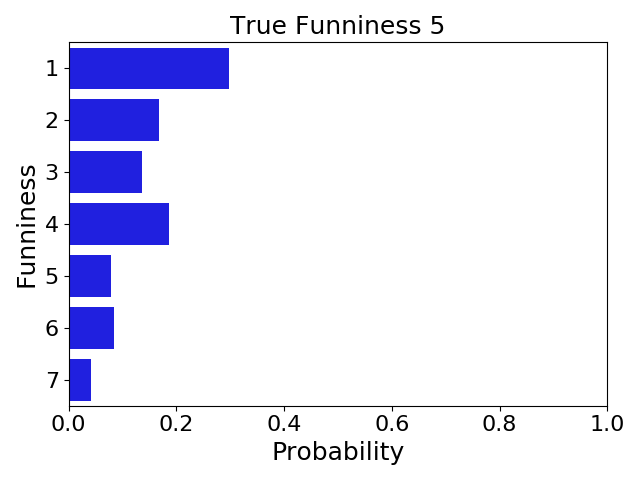
\includegraphics[width=1.0\textwidth]{graphics/detail/Test_for_Image_5}
\end{subfigure}\quad
\begin{subfigure}[b]{0.45\textwidth}
\centering
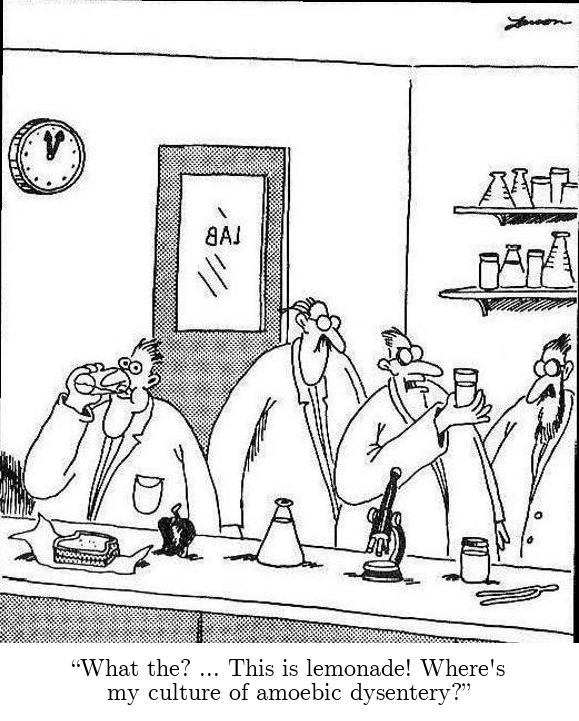
\includegraphics[width=0.9\textwidth,height=0.3\textheight,keepaspectratio]{graphics/detail/Test_for_Image_6_cartoon} \\
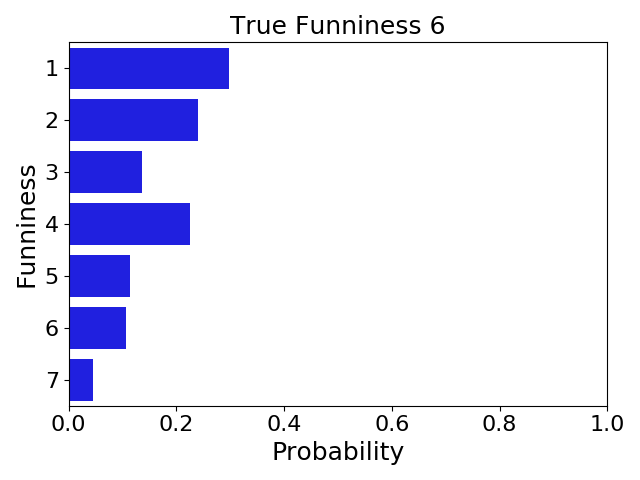
\includegraphics[width=1.0\textwidth]{graphics/detail/Test_for_Image_6}
\end{subfigure}

\begin{subfigure}[b]{0.45\textwidth}
\centering
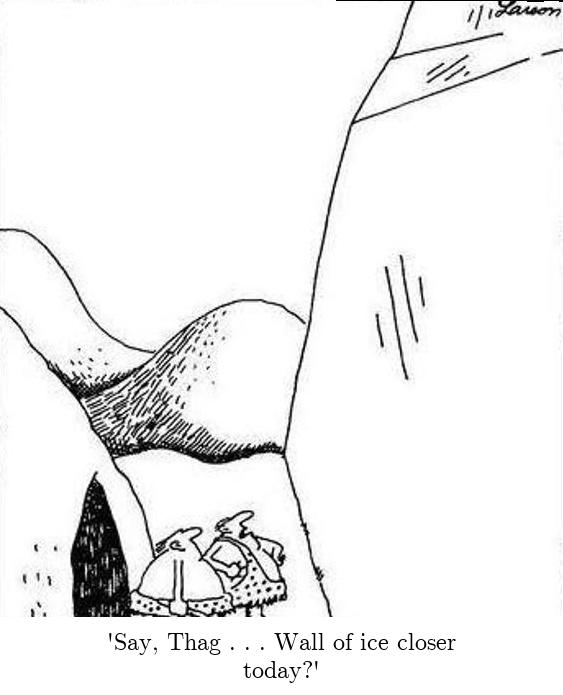
\includegraphics[width=0.9\textwidth,height=0.3\textheight,keepaspectratio]{graphics/detail/Test_for_Image_7_cartoon} \\
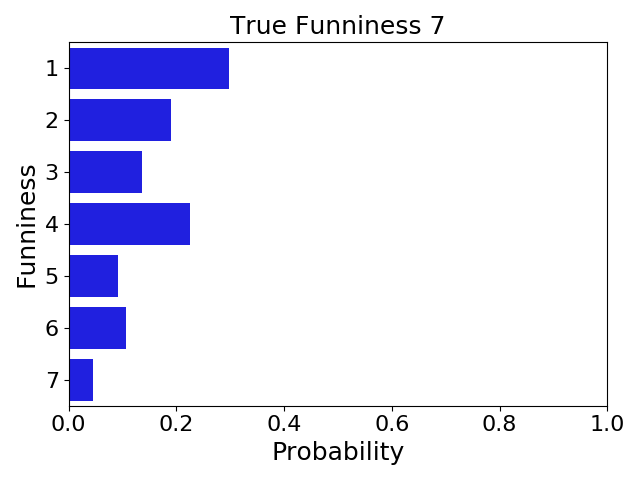
\includegraphics[width=1.0\textwidth]{graphics/detail/Test_for_Image_7}
\end{subfigure}\quad
\caption{Continued for the classes 5, 6 and 7.}
\label{fig:figdistr2}

\end{figure}

\begin{figure}
	\centering
  	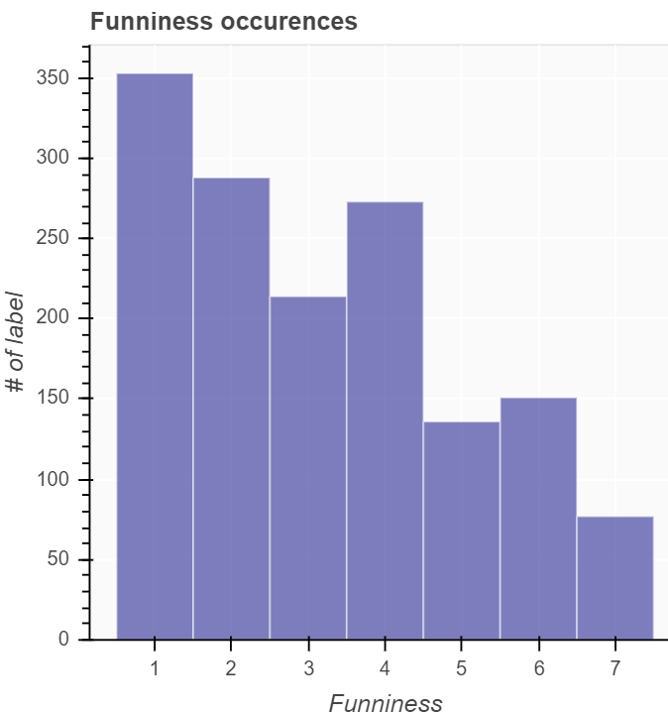
\includegraphics[width=0.75\textwidth]{graphics/label_distribution.png}
	\caption{The label distribution of the training set}
	\label{fig:labeldistr}
\end{figure}

\subsubsection{Confusion Matrix}
\begin{figure}
	\centering
  	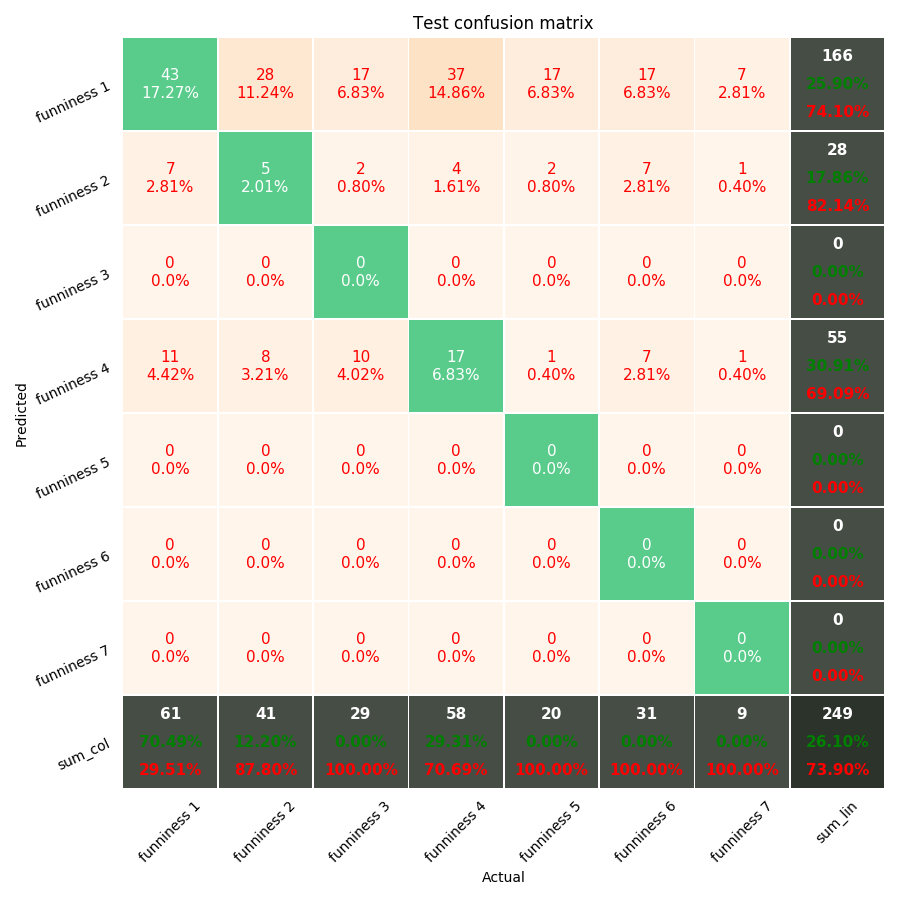
\includegraphics[width=1.0\textwidth]{graphics/transfer_confusion_test.png}
	\caption{Confusion Matrix of the transfer learning CNN (with data augmentation) on the test split}
	\label{fig:confusionmatrixtransferlearningtest}
\end{figure}

\begin{figure}
	\centering
  	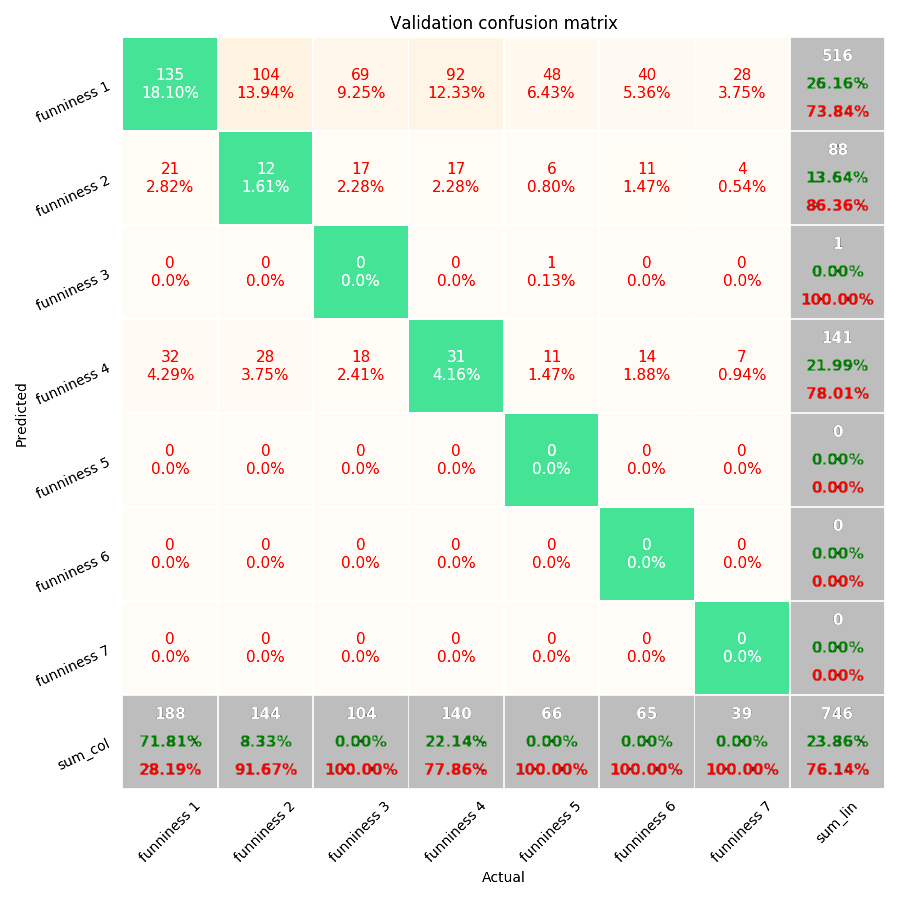
\includegraphics[width=1.0\textwidth]{graphics/transfer_confusion_val.png}
	\caption{Confusion Matrix of the transfer learning CNN (with data augmentation) on the validation split}
	\label{fig:confusionmatrixtransferlearningval}
\end{figure}

One can clearly see that for both the validation and test split the model learned to approximate the label distribution, instead of learning to generalize the underlying structure. The three most frequent funniness classes (1, 4 and 2) are the only ones the model predicts and are therefore by chance correct. Other classes are not predicted at all by the classifier. This motivated the design of the two stage model, where specific models are trained for each funniness class.


\subsection{Transfer Learned Object Detection}

The result of the object detection approach are incomparable to the other results, as it was not implemented far enough to return any labels. It was not further developed, as the predicted objects for each object were essentially random.

\subsection{ELMo Pretrained Model}

Based on the pretrained ELMo model this model initially looked the most promising, as it
achieved the highest validation accuracy. Unfortunately this was only due to overfitting,
as during test phase the performance dropped.

Most likely a problem of this approach is that many insider jokes are lost, due to the fact
that the pretrained vocabulary of the ELMo model does not contain many of them, so
they can not be used by our model. For example the word "Thag" which is one of the most frequent terms for cartoons with funniness 7 is not in the ELMo vocabulary and therefore ignored.

\subsection{AutoML Model}
Initially, when testing on the validation set, the TFIDF configuration looked very promising, as it achieved top results with a very simple feature representation. The test set
revealed overfitting. The ELMo feature representation performed worse in both settings.
Since the TFIDF feature representation would not have relied on a pre-trained vocabulary
it would not have suffered by the problem of domain specific words.

For this experiment the library hyperopt-sklearn \cite{hyperopt} was used, as it accomplishes state-of-the-art AutoML performance.

\subsection{Two Stage Model}
The Two Stage Models is not better than the average baseline. The idea of trying to avoid overfitting by using multiple classifiers for each funniness did not work as expected.

Combining the visual and text information did improve the results, but not significantly. The MAE
score is on par with the baseline, while still beating it at the accuracy score. This improvement is still very weak.
understands humor.

One problem identified was the fact, that the images contained much more data compared to the punchlines. To tackle this problem, the idea was to use a deep autoencoder. This reduces the feature size of the images significantly. But against our expectation it did not improve the results compared to previous attempts.

When comparing the MAE of the Two stage model (figure [\ref{twostagemae}]) an interesting phenomena can be observed: Even though the performance is very similar to the average baseline, the actual MAEs per class are different. This means that the model does not simply return the average funniness, but does something else.

\begin{figure}
\centering
\begin{tabular}{|l|l|l|l|l|l|l|l|} 
\hline
\textbf{Funniness} 	& \textbf{1}	& \textbf{2}	& \textbf{3}	& \textbf{4}	& \textbf{5}	& \textbf{6}	& \textbf{7}  \\ 
\hline
Two Stage Model     & 2.42			&  1.57			& 0.97			& 0.8			& 1.53			& 2.28			& 3.64   \\
Baseline Average    & 2.21			& 1.21			& 0.21			& 0.79			& 1.79			& 2.79			& 3.79 \\	
\hline
\end{tabular}
\caption{MAE per class}
\label{twostagemae}
\end{figure}

A confusion matrix of each classifier in the first stage reveals whether this approach could be effective. If all classifiers have a reasonable accuracy the second decision stage has a higher chance of predicting the correct class. If the first stage only returns noise the second stage would not be able to beat the average baseline.

It seems that the first stage is not effective in doing so. For funniness 3, 4, 5, 6 and 7 there is no true negative, which means that the model for this class only learns to always return 1.

\begin{figure}
\centering

\begin{subfigure}[b]{0.45\textwidth}
\centering
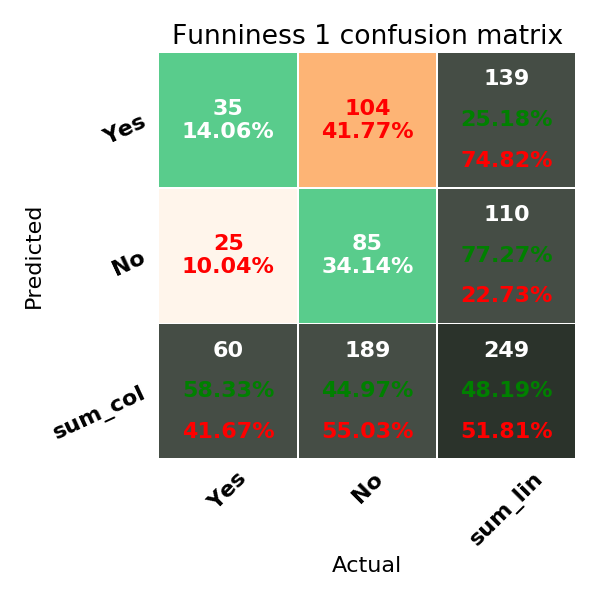
\includegraphics[width=0.9\textwidth,height=0.3\textheight,keepaspectratio]{graphics/twostageperf/funniness1}
\end{subfigure}\quad
\begin{subfigure}[b]{0.45\textwidth}
\centering
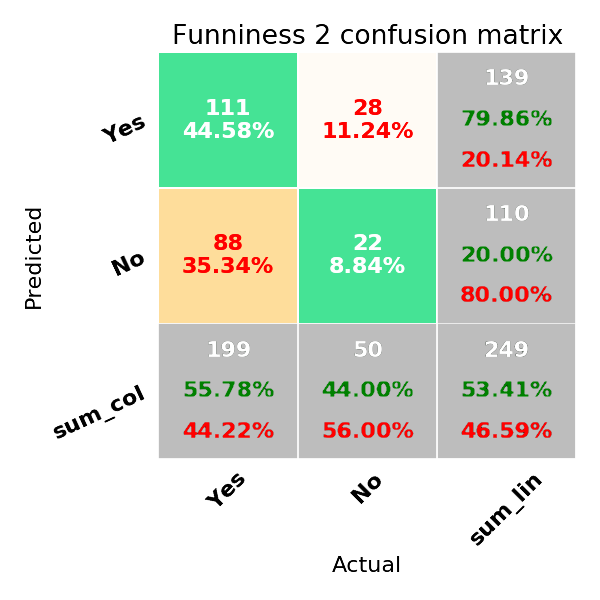
\includegraphics[width=0.9\textwidth,height=0.3\textheight,keepaspectratio]{graphics/twostageperf/funniness2}
\end{subfigure}

\begin{subfigure}[b]{0.45\textwidth}
\centering
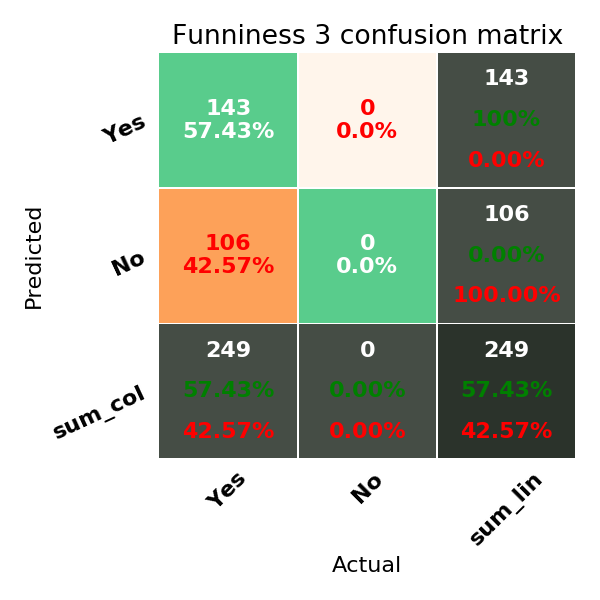
\includegraphics[width=0.9\textwidth,height=0.3\textheight,keepaspectratio]{graphics/twostageperf/funniness3}
\end{subfigure}\quad
\begin{subfigure}[b]{0.45\textwidth}
\centering
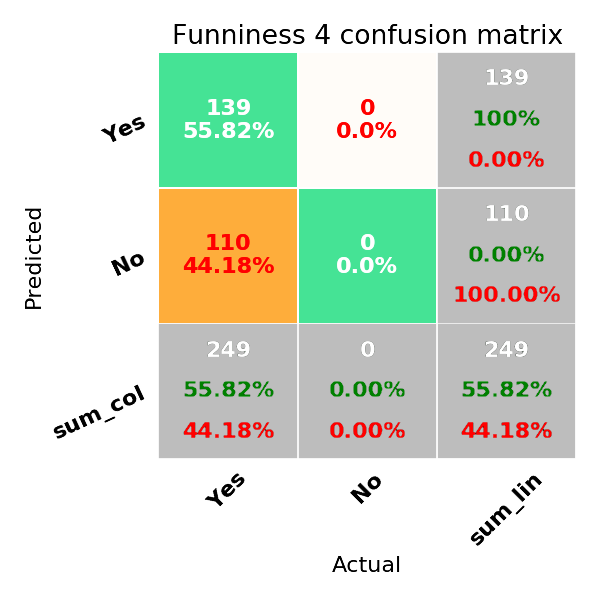
\includegraphics[width=0.9\textwidth,height=0.3\textheight,keepaspectratio]{graphics/twostageperf/funniness4}
\end{subfigure}

\begin{subfigure}[b]{0.45\textwidth}
\centering
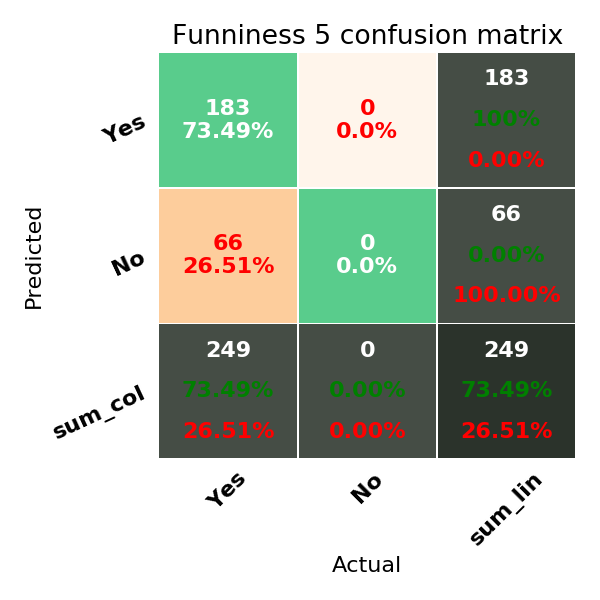
\includegraphics[width=0.9\textwidth,height=0.3\textheight,keepaspectratio]{graphics/twostageperf/funniness5}
\end{subfigure}\quad
\begin{subfigure}[b]{0.45\textwidth}
\centering
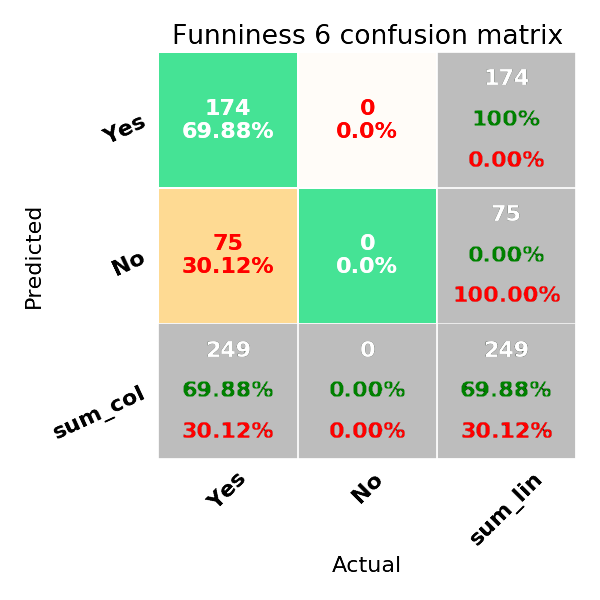
\includegraphics[width=0.9\textwidth,height=0.3\textheight,keepaspectratio]{graphics/twostageperf/funniness6}
\end{subfigure}


\begin{subfigure}[b]{0.45\textwidth}
\centering
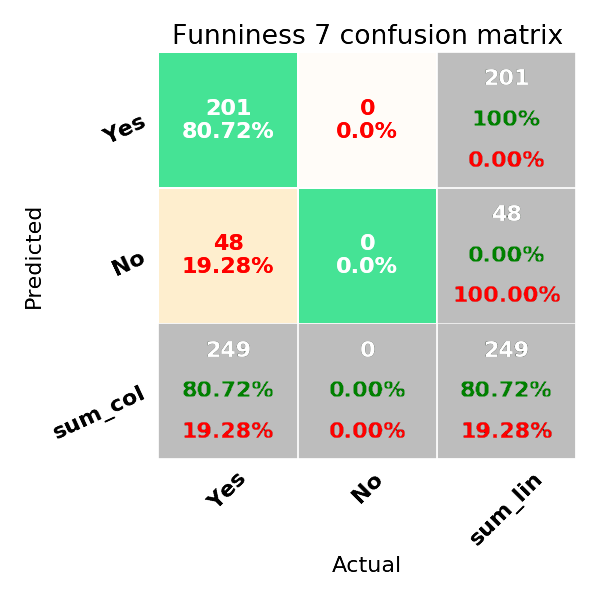
\includegraphics[width=0.9\textwidth,height=0.3\textheight,keepaspectratio]{graphics/twostageperf/funniness7}
\end{subfigure}


\caption{Confusion Matrices for first stage.}
\label{fig:firststageconf}

\end{figure}


\subsection{Autoencoder}

The goal of the auto encoder using the deep convolutional architecture is to reduce the dimensionality of the images, while still maintaining the important characteristics of the original cartoons. 

Comparing the reconstructed cartoon with the original cartoon reveals that the autoencoder looses important semantic information which could be crucial for understanding humor. For example the facial expressions are lost, as well as many other high frequency details. For example the native American lying on the floor is not recognizable anymore. 

These details seem to be very important for the funniness classification task and if missing cause the image data to be not more than additional noise, which is probably the reason why the two stage model with autoencoded cartoons performs worse.

\begin{figure}
	\centering
  	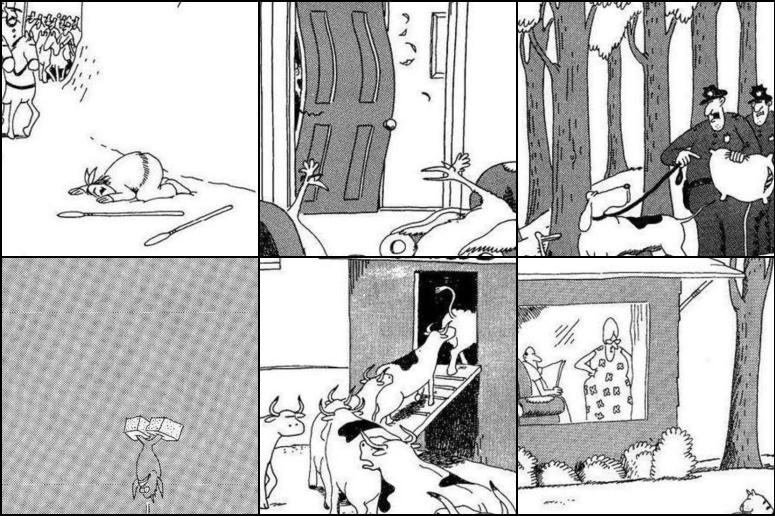
\includegraphics[width=1.0\textwidth]{graphics/autoencoder_original.png}
	\caption{Original Cartoons}
	\label{fig:autoencoderimageoriginal}
\end{figure}

\begin{figure}
	\centering
  	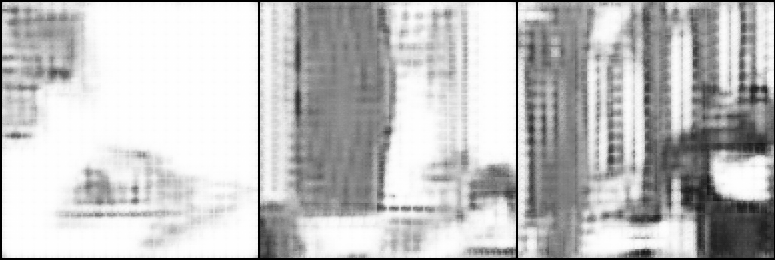
\includegraphics[width=1.0\textwidth]{graphics/autoencoder_final.png}
	\caption{Results after applying encoder and decoder}
	\label{fig:autoencoderresults}
\end{figure}

\section{Results}

The following sections show the achieved performance for each experiment of the validation
and test phase. Additionally the training runtime is also listed.


\subsection{Validation Results}

For a detailed table of validation performance of selected models, please refer to figure [\ref{fig:valperformance}]. The ELMo based model achieved on this subset the highest accuracy, while the Two Stage Model achieved the best mean Absolute Error. Both models only use the text data and discard the visual information entirely.

\begin{figure}
\begin{tabular}{|l|l|l|l|l|}
\hline
\textbf{Experiment}                                                                       & \textbf{\begin{tabular}[c]{@{}l@{}}Validation\\   MAE\end{tabular}} & \textbf{\begin{tabular}[c]{@{}l@{}}Validation\\   Accuracy\end{tabular}} & \textbf{Text} & \textbf{Visual} \\ \hline
Baseline Most Frequent                                                                    & 2.14                                                                & 25.20\%                                                                  &               &                 \\
Baseline Average                                                                          & 1.53                                                                & 13.94\%                                                                  &               &                 \\
Baseline Random                                                                           & 2.33                                                                & 13.81\%                                                                  &               &                 \\
Baseline Stratified                                                                       & 2.03                                                                & 16.62\%                                                                  &               &                 \\
Simple CNN                                                                                & 2.14                                                                & 25.20\%                                                                  &               & \cmark               \\
Transfer Learning CNN                                                                      & 1.88                                                                & 25.53\%                                                                  &               & \cmark               \\
\begin{tabular}[c]{@{}l@{}}Transfer Learning CNN (with\\   data augmentation)\end{tabular} & 1.96                                                                & 23.86\%                                                                  &               & \cmark               \\
ELMo                                                                                      & 1.81                                                                & \textbf{26.81\%}                                                                  & \cmark             &                 \\
AutoML Model with ELMo Vectors                                                            & 2                                                                   & 25.87\%                                                                  & \cmark             &                 \\
\begin{tabular}[c]{@{}l@{}}AutoML Model with TFIDF\\   Vectors\end{tabular}               & 2.05                                                                & 26.76\%                                                                  & \cmark             &                 \\
Two Stage Model                                                                           & \textbf{1.52}                                                                & 18.10\%                                                                  & \cmark             & \\
Two Stage Model with Cartoons                                                             & 1.55                                                                & 15.68\%                                                                  & \cmark             & \cmark               \\
\begin{tabular}[c]{@{}l@{}}Two Stage Model with\\   Autoencoded Cartoons\end{tabular}     & 1.62                                                                & 15.82\%                                                                  & \cmark             & \cmark               \\ \hline
\end{tabular}
\caption{Model performances on the validation set.}
\label{fig:valperformance}
\end{figure}

\subsection{Test Results}

The results at figure [\ref{fig:testperformance}] show the performance of the models for the test set. Compared to the validation set the best performing models change: The model which maximizes the accuracy measure is now using the visual data, namely the transfer learning CNN on the data augmented test set. Also the two stage model without cartoon data seems to generalize slightly better.

\begin{figure}
\begin{tabular}{|l|l|l|l|l|}
\hline
\textbf{Experiment}                                                                       & \textbf{Test MAE} & \textbf{Test Accuracy} & \textbf{Text} & \textbf{Visual} \\ \hline
Baseline Most Frequent                                                                    & 2.26              & 24.50\%                &               &                 \\
Baseline Average                                                                          & \textbf{1.57}              & 11.65\%                &               &                 \\
Baseline Random                                                                           & 2.17              & 13.65\%                &               &                 \\
Baseline Stratified                                                                       & 2.22              & 14.46\%                &               &                 \\
Simple CNN                                                                                & 2.26              & 24.50\%                &               & \cmark               \\
Transfer Learning CNN                                                                      & 1.96              & 24.90\%                &               & \cmark               \\
\begin{tabular}[c]{@{}l@{}}Transfer Learning CNN (with\\   data augmentation)\end{tabular} & 2.01              & \textbf{26.10\%}                &               & \cmark               \\
ELMo                                                                                      & 1.84              & 25.70\%                & \cmark             &                 \\
AutoML Model with ELMo Vectors                                                            & 2.12              & 24.50\%                & \cmark             &                 \\
\begin{tabular}[c]{@{}l@{}}AutoML Model with TFIDF\\   Vectors\end{tabular}               & 2.23              & 24.90\%                & \cmark             &                 \\
Two Stage Model                                                                           & 1.6               & 18.80\%                & \cmark             &                 \\
Two Stage Model with Cartoons                                                             & \textbf{1.57}              & 16.06\%                & \cmark             & \cmark               \\
\begin{tabular}[c]{@{}l@{}}Two Stage Model with\\   Autoencoded Cartoons\end{tabular}     & 1.58              & 14.46\%                &\cmark             & \cmark              \\
\hline
\end{tabular}
\caption{Model performances on the test set.}
\label{fig:testperformance}
\end{figure}

\subsection{Training Duration}

Figure [\ref{trainingruntime}] shows the training durations of each experiment. A general trend, is that the text based models (ELMo, Two Stage Model) train significantly faster than the visual based models (Simple CNN, Transfer Learning CNN, Two Stage Model with Cartoons). This can be explained by the size of the input vector for the neural network. The data for the text representation is denser compared to the representation of images.

\begin{figure}
\centering
\begin{tabular}{|l|l|} 
\hline
\textbf{Experiment}                                    & \textbf{Train Duration}  \\ 
\hline
Baseline Most Frequent                        & \textless{}1s   \\
Baseline Average                              & \textless{}1s   \\
Baseline Random                               & \textless{}1s   \\
Baseline Stratified                           & \textless{}1s   \\
Simple CNN                                    & 7m 50s          \\
Tranfer Learning CNN                          & 15m 45s         \\
Tranfer Learning CNN (with data augmentation) & 9m 52s          \\
ELMo                                          & 4m 39s          \\
AutoML Model with ELMo Vectors                & 29m 7s          \\
AutoML Model with TFIDF Vectors               & 24m 20s         \\
Two Stage Model                               & 8m 42s          \\
Two Stage Model with Cartoons                 & 39m 42s         \\
Autoencoder                                   & 32m 34s         \\
Two Stage Model with Autoencoded Cartoons     & 15m 23s         \\
\hline
\end{tabular}
\caption{Training runtime of each experiment}
\label{trainingruntime}
\end{figure}

\chapter {Conclusion}

In general no model really learns to generalize the humor of Gary Larson. There has been no significant improvement compared to the baselines. Further research could reveal significant insights on how human humor works.

Potential causes can not be attributed to exactly one issue. One reason is most certainly, that the problem space is not sufficiently grasped by the data set. As most deep learning data sets are many order of magnitudes larger, while the task at hand is arguably easier (For example: CIFAR 10 data set \cite{dogsvscats}) than humor classification. Current techniques of transfer learning are not sufficient to solve this issue. Most certainly once more sophisticated transfer learning techniques have been established, solving this problem could be more feasible. 

One could also argue that the problem itself is flawed. Letting a human rate a
cartoon is very subjective and likely depends on many factors. For example: Current mood, whether the person has already seen the cartoon, time of day and also the exact reason for performing the annotation. It could be that these factors outweigh the true humor, which makes it impossible to reproduce the original ratings. To answer this question an additional experiment could be performed: After some time after the initial ratings were performed, the same person rates the cartoons again. If the ratings are not reproducible by the same annotator, then it seems to be impossible for a deep learning based model.

%\chapter{Introduction}
%\todo{Enter your text here.}

%\chapter{Additional Chapter}
%\todo{Enter your text here.}

\backmatter

% Use an optional list of figures.
\listoffigures % Starred version, i.e., \listoffigures*, removes the toc entry.

% Use an optional list of tables.
% \cleardoublepage % Start list of tables on the next empty right hand page.

% \listoftables % Starred version, i.e., \listoftables*, removes the toc entry.

% Use an optional list of alogrithms.
% \listofalgorithms
% \addcontentsline{toc}{chapter}{List of Algorithms}

% Add an index.
% \printindex

% Add a glossary.
% \printglossaries

% Add a bibliography.
\bibliographystyle{abbrv}
\bibliography{citations}

\end{document}